The classical lost lepton method is a validated method that was used in analysis of the 2015 data~\cite{PhysRevD.96.012004}. Although the analysis of the 2016 data uses the simulation based translation factor method for the background estimation for \ttbar, single top and W+jets, the classical method is still an important cross check method. 

The name (lost lepton) of the background is interesting. On one hand, lost lepton indicates leptons that are lost because they are not in the acceptance, not reconstructed or not isolated. On the other hand, a lost lepton is like a lost boy. The boy becomes crazy and finally is misidentified as a jet. The expected numbers of lost lepton events are categorized in Table~\ref{tab:nexpLL}. The numbers of not accepted and not isolated events for muons and electrons are very similar. This is expected because of lepton flavor symmetry among \ttbar decay channels. However, the numbers of not reconstructed muon and electron are very different. The difference comes from the nature of detector: the muons detected by muon system have higher reconstruction efficiencies than electrons in ECAL. 

\begin{table}[htbp]
\fontsize{10 pt}{1.2 em}
\caption{Number of expected lost lepton events (not isolated, not identified/reconstructed and out of the acceptance) in \ttbar, single top and W+jets simulation events, for a luminosity of $35.9$~fb$^{-1}$.} 
\begin{center}
\begin{tabular}{|c|c|c|c|}
\hline
          & iso  & id   & acc \\
\hline
muons     & $139.6\pm16.4$ & $71.3\pm12.5$ & $707.7\pm38.2$ \\
electrons & $148.8\pm17.8$ & $305.2\pm25.3$ & $692.8\pm38.6$ \\
\hline\end{tabular}
\end{center}
\label{tab:nexpLL}
\end{table}

\paragraph{Description of the method}

The lepton identification chain is shown in Fig~\ref{fig:llmethod}. The event will satisfy the lepton veto if the lepton in the event is out of acceptance, not identified, or not isolated. Therefore, we can calculate the acceptance, identification and isolation efficiency in the single lepton control sample in simulation. And then, apply those efficiencies to the single lepton data sample with a model to estimate the lost lepton yield in the search region. 

\begin{figure}[htbp]
\begin{center}
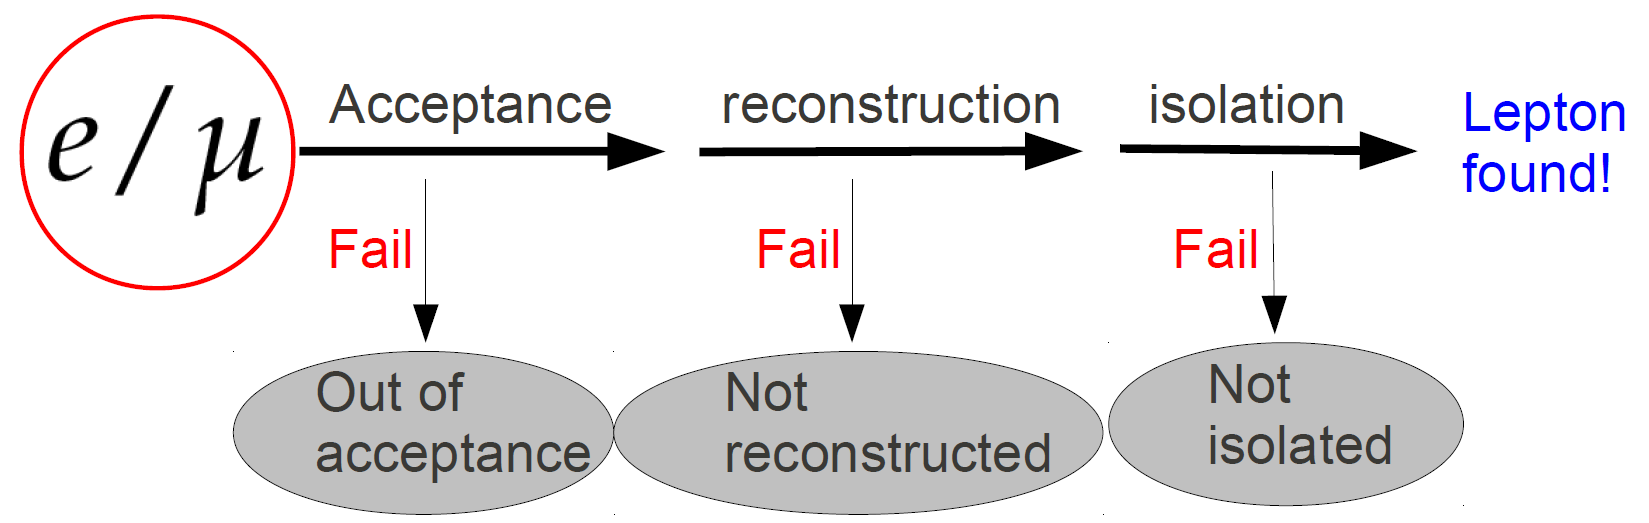
\includegraphics[width=0.55\textwidth]{sections/mc4/Backgrounds/LostLepton/figures/lepton_veto_sketch.png}
\end{center}
\caption{Sketch of the requirements electrons and muons from $W$ decays must meet in order to be rejected by the explicit lepton veto.}
\label{fig:llmethod}
\end{figure}

However, the single lepton control sample can have a large signal contamination for some search bins, i.e., a large contribution of signal events. To reduce the contamination, only events with lepton transverse mass smaller than 100 GeV are considered. The lepton $m_{\rm T}$ is defined in Eq~\ref{eq:MTW}:
\begin{equation}
m_{\rm T} = \sqrt{2 p_{\rm T}(lepton) E^{\rm miss}_{\rm T} (1 - \cos(\Delta \Phi))},
\label{eq:MTW}
\end{equation}
where $\Delta \Phi$ is the distance in $\Phi$ between the muon and the $\MET$. For the electroweak control sample $\MET$ originates from the neutrino, $m_{\rm T}$ represents the transverse $W$-mass ($M_{T}^{W}$), and therefore the distribution falls sharply above $80$~GeV. To compensate for the loss in efficiency due to the $m_{\rm T}$ selection requirement, a correction factor is added in the lost lepton prediction model. 

We also need to consider the events with multiple lost leptons. Here we only estimate a part of the first-order effect: di-muon, di-electron and one electron plus one muon events. Events with a higher number of leptons are not considered. The simplification is reasonable since the correction factor is very close to 1.

As mentioned in the event selection section, an isolated track veto is used to reject 1-prong hadronic tau events. An overall correction factor is applied to account for this selection requirement. 

To summarize, the predicted number of \ttbar, $W$+jets and single top events with lost leptons, $N_{LostLepton}$ contributing to the search sample can be calculated by Eq~\ref{eq:lostleptonequation}:

\begin{equation}
N_{LostLepton}= \sum_{CS} (\sum_{i={e,\mu}}({F_{ISO}}^{i}+{F_{ID}}^{i}+{F_{Acc}}^{i}) \times F_{dilepton}^{i}) \times E_{Mtw} \times \epsilon_{isotrack},
\label{eq:lostleptonequation}
\end{equation}
where $\sum_{CS}$ is the sum over the events in the control sample after the baseline selection, ${F_{ISO}}^{i}$, ${F_{ID}}^{i}$ and ${F_{Acc}}^{i}$ are factors converting the number of events in the control sample to the number of lost lepton events due to respectively isolation, reconstruction or acceptance criteria, $F_{dilepton}^{i}$ is the correction factor for the di-lepton contribution, $E_{Mtw}$ is the correction factor for the $M_{T}^{W}$ selection requirement and $\epsilon_{isotrack}$ is the correction factor to compensate for the isolated track veto. The simulation based factors are described in the remainder of this section.

The control sample is normalized to compensate for the reduction of efficiency because of the $M_{T}^{W}<100$~GeV requirement, as illustrated in Table~\ref{tab:mtw}, which shows the $M_{T}^{W}$ correction factors, obtained from simulation, as a function of muon $p_{T}$. 

\begin{table}[htbp]
\fontsize{10 pt}{1.2 em}
\caption{$M_{T}^{W}$ correction factors obtained from \ttbar, single top and W$+$jets simulation, after baseline selection. Only statistical uncertainties are shown.}
\begin{center}
\begin{tabular}{|c|c|c|c|c|c|c|c|}
\hline
\specialcell{Muon \\ $p_T$ [GeV]} & 10-20 & 20-30 & 30-40 & 40-50 & 50-70 & 70-100 & $>100$ \\
\hline
\specialcell{$M_{T}^{W}$ \\ factor} & \specialcell{1.04\\ $\pm$0.01} & \specialcell{1.06\\ $\pm$0.01} & \specialcell{1.07\\ $\pm$0.01} & \specialcell{1.09\\ $\pm$0.01} & \specialcell{1.11\\ $\pm$0.01} & \specialcell{1.19\\ $\pm$0.01} & \specialcell{1.66\\ $\pm$0.02} \\
\hline
\end{tabular}
\end{center}
\label{tab:mtw}
\end{table}

The control sample is weighted according to the lepton isolation efficiency in order to model the non-isolated leptons in the signal region (${F_{ISO}}^{i}$). 
The calculation is for muons and electrons depending on the superscript:
\begin{equation}
{F_{ISO}}^{e/\mu} =  \frac{1-\epsilon_{\rm ISO}^{e/\mu}}{\epsilon_{\rm ISO}^{\mu}} \cdot \frac{\epsilon^{e/\mu}_{\rm ID}}{\epsilon^{\mu}_{\rm ID}} \cdot \frac{\epsilon^{e/\mu}_{\rm Acc}}{\epsilon^{\mu}_{Acc}}.
\label{eq:isolation}
\end{equation}
To model the sample containing no identified electron or muons in the signal region, the control sample is weighted as follows:
\begin{equation}
{F_{ID}}^{e/\mu} = \frac{1}{\epsilon_{\rm ISO}^{\mu}}\cdot \frac{1-\epsilon_{\rm ID}^{e/\mu}}{\epsilon_{\rm ID}^{\mu}}  \cdot \frac{\epsilon^{e/\mu}_{\rm Acc}}{\epsilon^{\mu}_{\rm Acc}}.
\label{eq:id}
\end{equation}

The isolation and reconstruction efficiencies as well as the acceptance are obtained from simulated \ttbar and W$+$jets events. They are measured using reconstructed muons and electrons after the baseline selection and parameterized as a function of the muon $p_T$ and the activity around the lepton, defined as the sum of the $p_{T}$'s of all PF particle candidates in an annulus outside a standard isolation divided by the $p_T$ of the lepton:
\begin{equation}
\textit{$A_{\mu/e}$}=\left(\sum^{R_\texttt{miniIso}<r<0.4}_\texttt{PFcands} p_\text{T}\right) / p_\text{T}(lep) \; .
\label{eq:activity}
\end{equation}

The lepton isolation and reconstruction efficiencies are analysis independent. Therefore, they are calculated without the baseline selection. They are shown in Figs~\ref{fig:muoneffiso},~\ref{fig:eleeffiso},~\ref{fig:muoneffreco} and~\ref{fig:eleeffreco}.

\begin{figure}[hptb]
\begin{center}
\begin{tabular}{c}
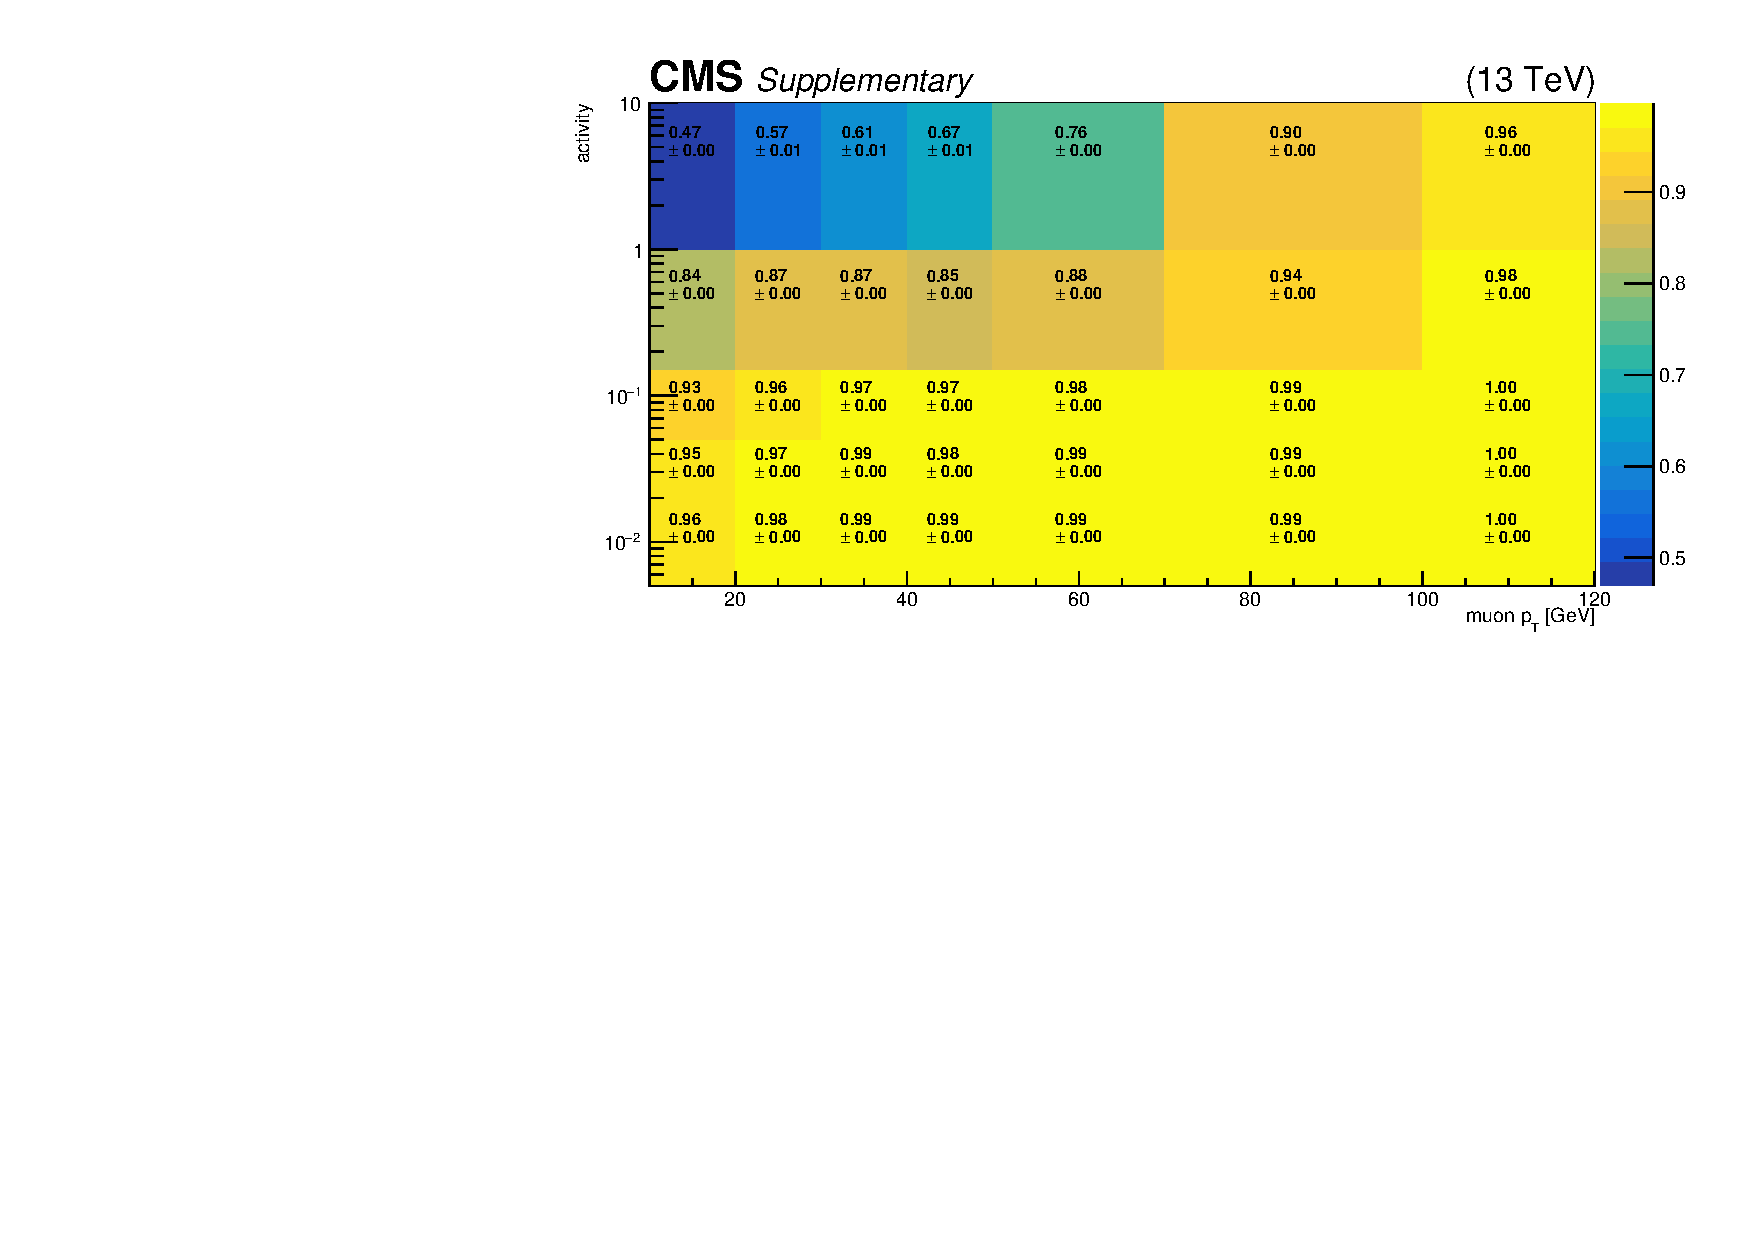
\includegraphics[width=1.0\textwidth]{sections/mc4/Backgrounds/LostLepton/figures/v3_2d_effs_mus_iso_no_baseline.pdf}
\end{tabular}
\end{center}
\caption{Muon isolation efficiencies as a function of the muon $p_T$ and the activity around the muon. Only statistical uncertainties are shown.}
\label{fig:muoneffiso}
\end{figure}

\begin{figure}[hptb]
\begin{center}
\begin{tabular}{c}
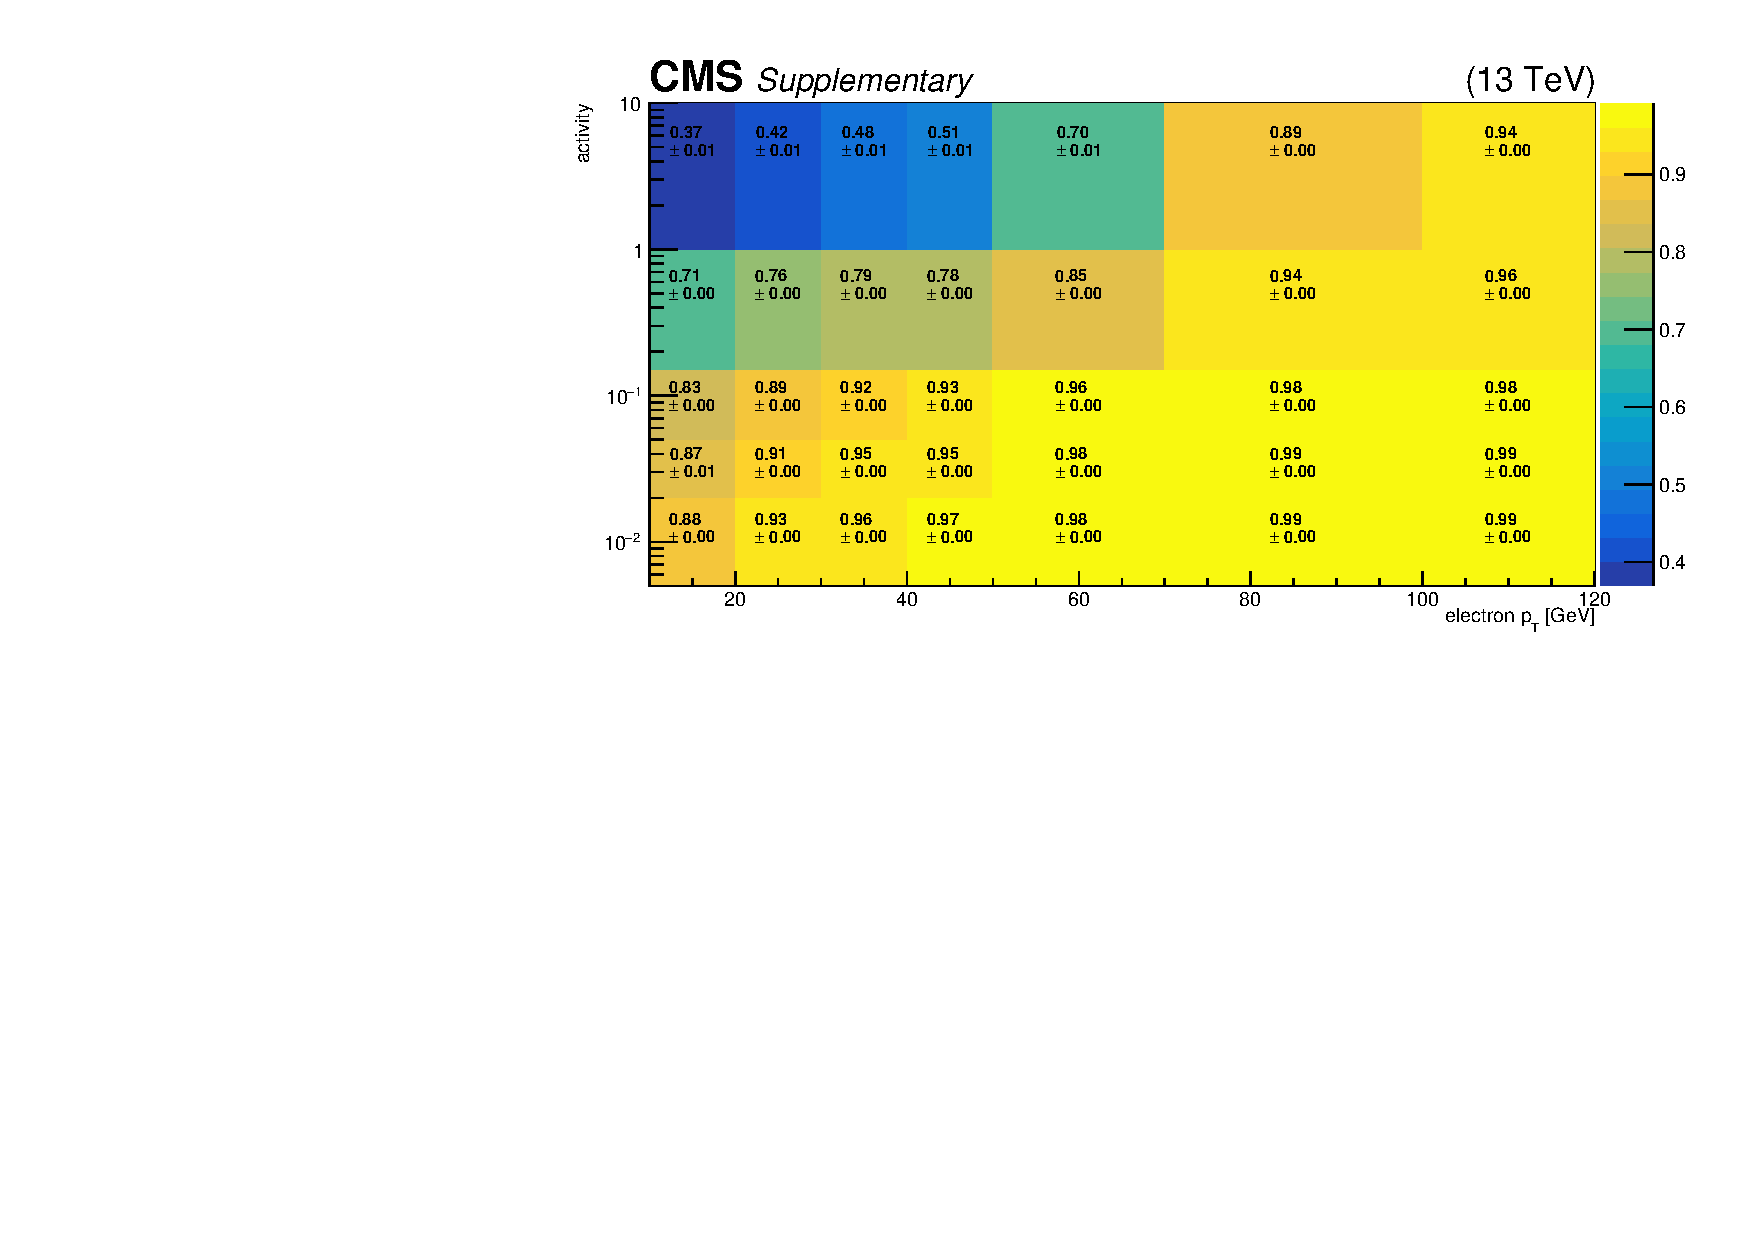
\includegraphics[width=1.0\textwidth]{sections/mc4/Backgrounds/LostLepton/figures/v3_2d_effs_els_iso_no_baseline.pdf}
\end{tabular}
\end{center}
\caption{Electron isolation efficiencies as a function of the electron $p_T$ and the activity around the electron. Only statistical uncertainties are shown.}
\label{fig:eleeffiso}
\end{figure}

\begin{figure}[hptb]
\begin{center}
\begin{tabular}{c}
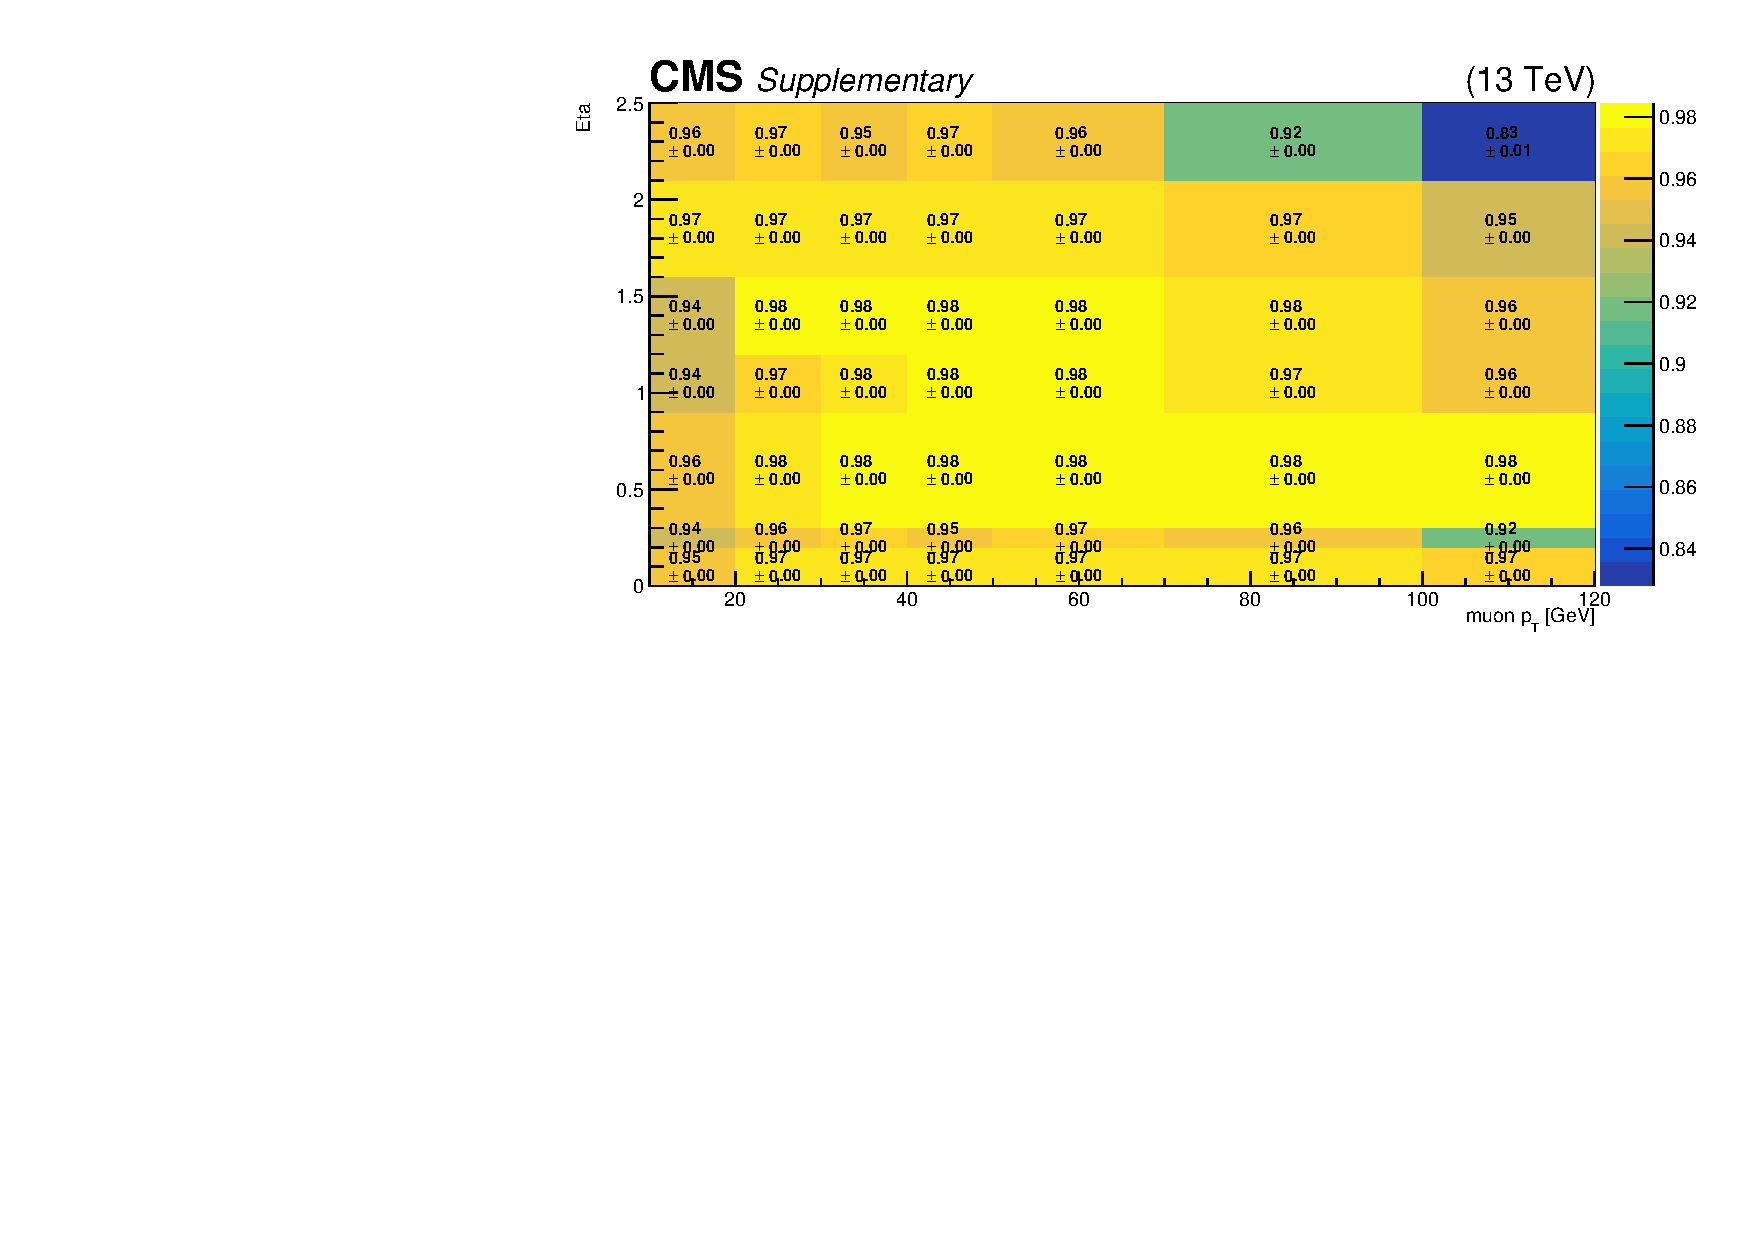
\includegraphics[width=1.0\textwidth]{sections/mc4/Backgrounds/LostLepton/figures/v3_2d_effs_mus_reco_no_baseline.pdf}
\end{tabular}
\end{center}
\caption{Muon reconstruction efficiencies as a function of the muon $p_T$ and Eta. Only statistical uncertainties are shown.}
\label{fig:muoneffreco}
\end{figure}

\begin{figure}[hptb]
\begin{center}
\begin{tabular}{c}
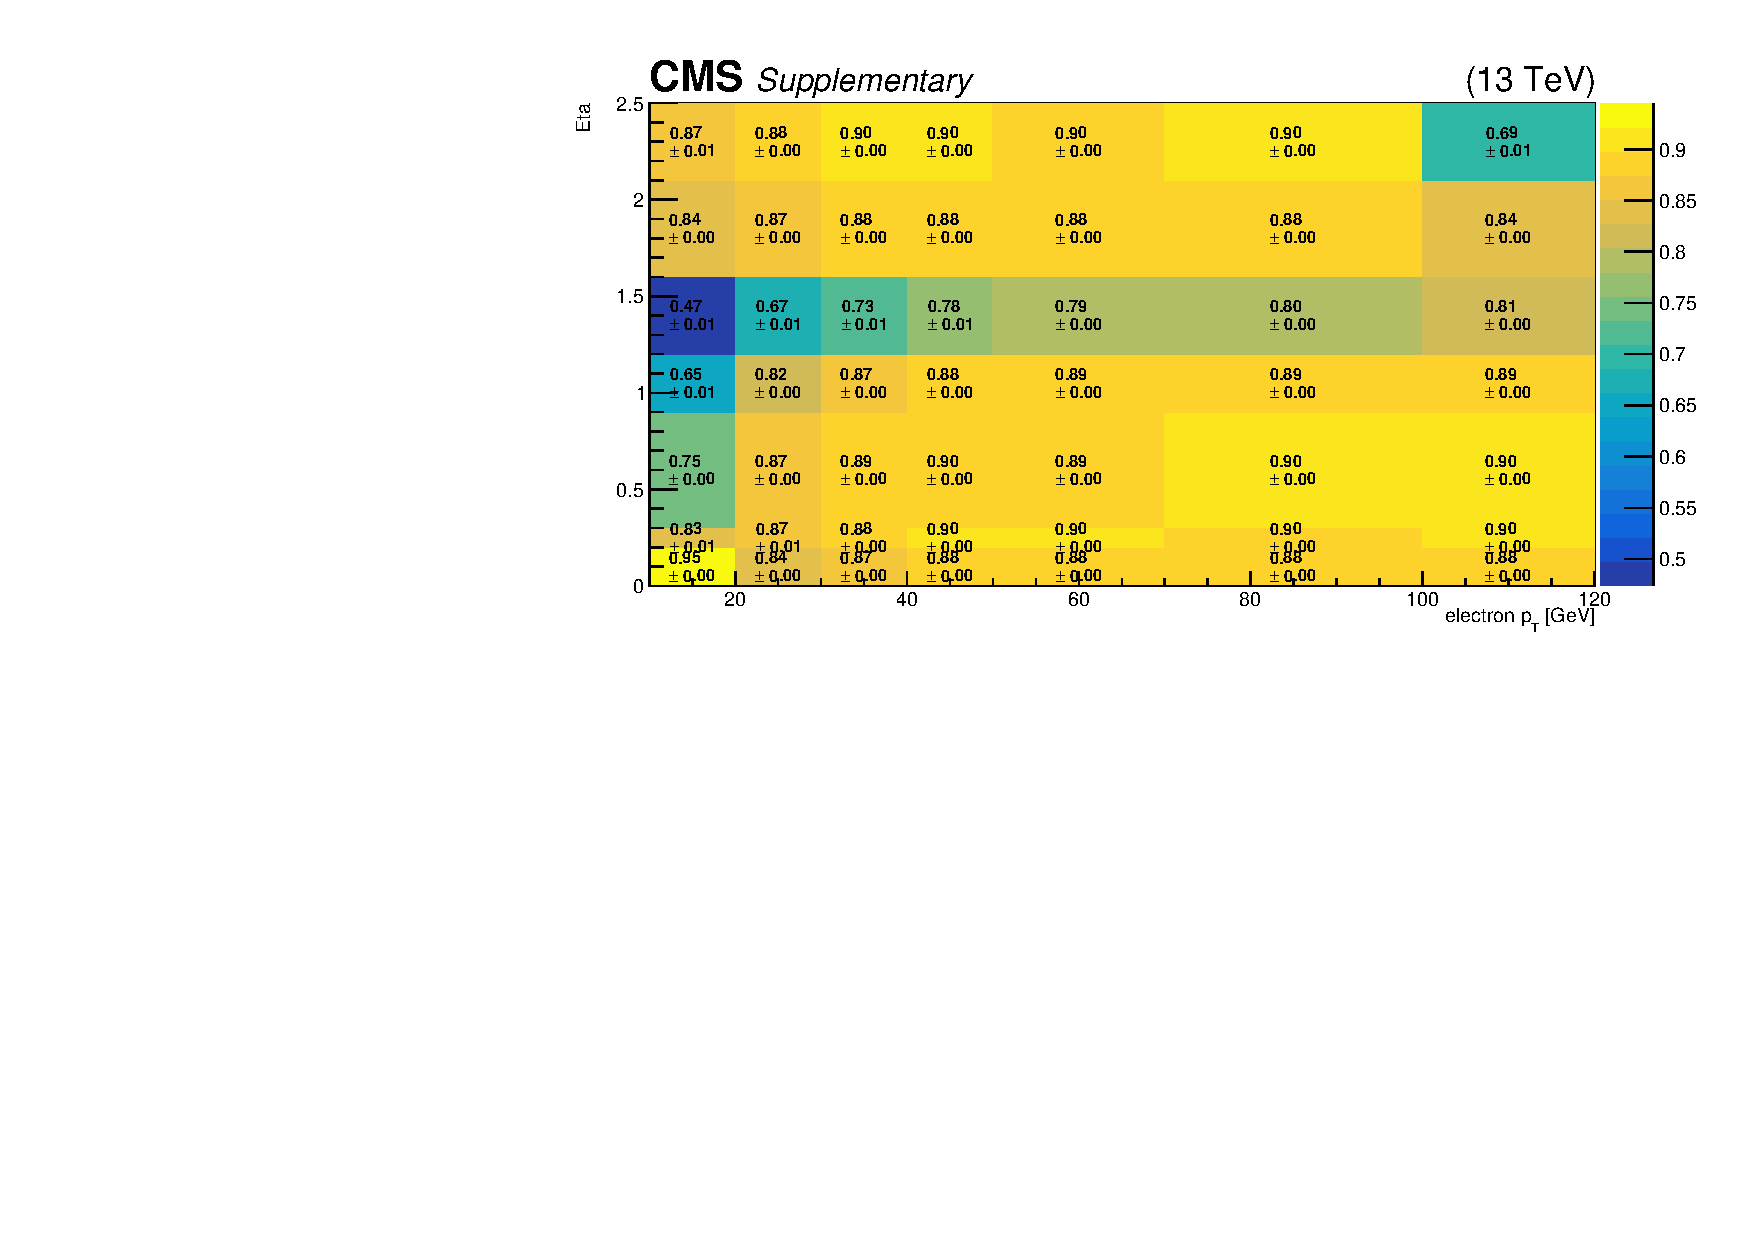
\includegraphics[width=1.0\textwidth]{sections/mc4/Backgrounds/LostLepton/figures/v3_2d_effs_els_reco_no_baseline.pdf}
\end{tabular}
\end{center}
\caption{Electron reconstruction efficiencies as a function of the electron $p_T$ and Eta. Only statistical uncertainties
are shown.}
\label{fig:eleeffreco}
\end{figure}

Another multiplicative factor to the number of control region events originates from leptons that 
are out of acceptance. Such events occur when leptons have a transverse 
momentum below the lepton veto $p_{T}$ threshold or when leptons are emitted in 
the forward region outside the $\eta$ acceptance. %, or when electrons are emitted in the transition region.
For example, leptons from leptonic-tau decays tend to have low 
momentum as well as neutrinos that contribute to the event \MET. 
This ${F_{Acc}}^{e/\mu}$ factor is modeled according to the following equation:
\begin{equation}
{F_{Acc}}^{e/\mu} = \frac{1}{\epsilon_{\rm ISO}^{\mu}}\cdot \frac{1}{\epsilon_{\rm ID}^{\mu}}  \cdot \frac{1 - \epsilon^{e/\mu}_{\rm Acc}}{\epsilon^{\mu}_{\rm Acc}}.
\label{eq:accept}
\end{equation}
The acceptance efficiencies are derived for each search bin 
from \ttbar and W$+$jets simulated events,
selected using the baseline criteria. 
They are shown in Fig~\ref{fig:acceptance}.

\begin{figure}[hptb]
\begin{center}
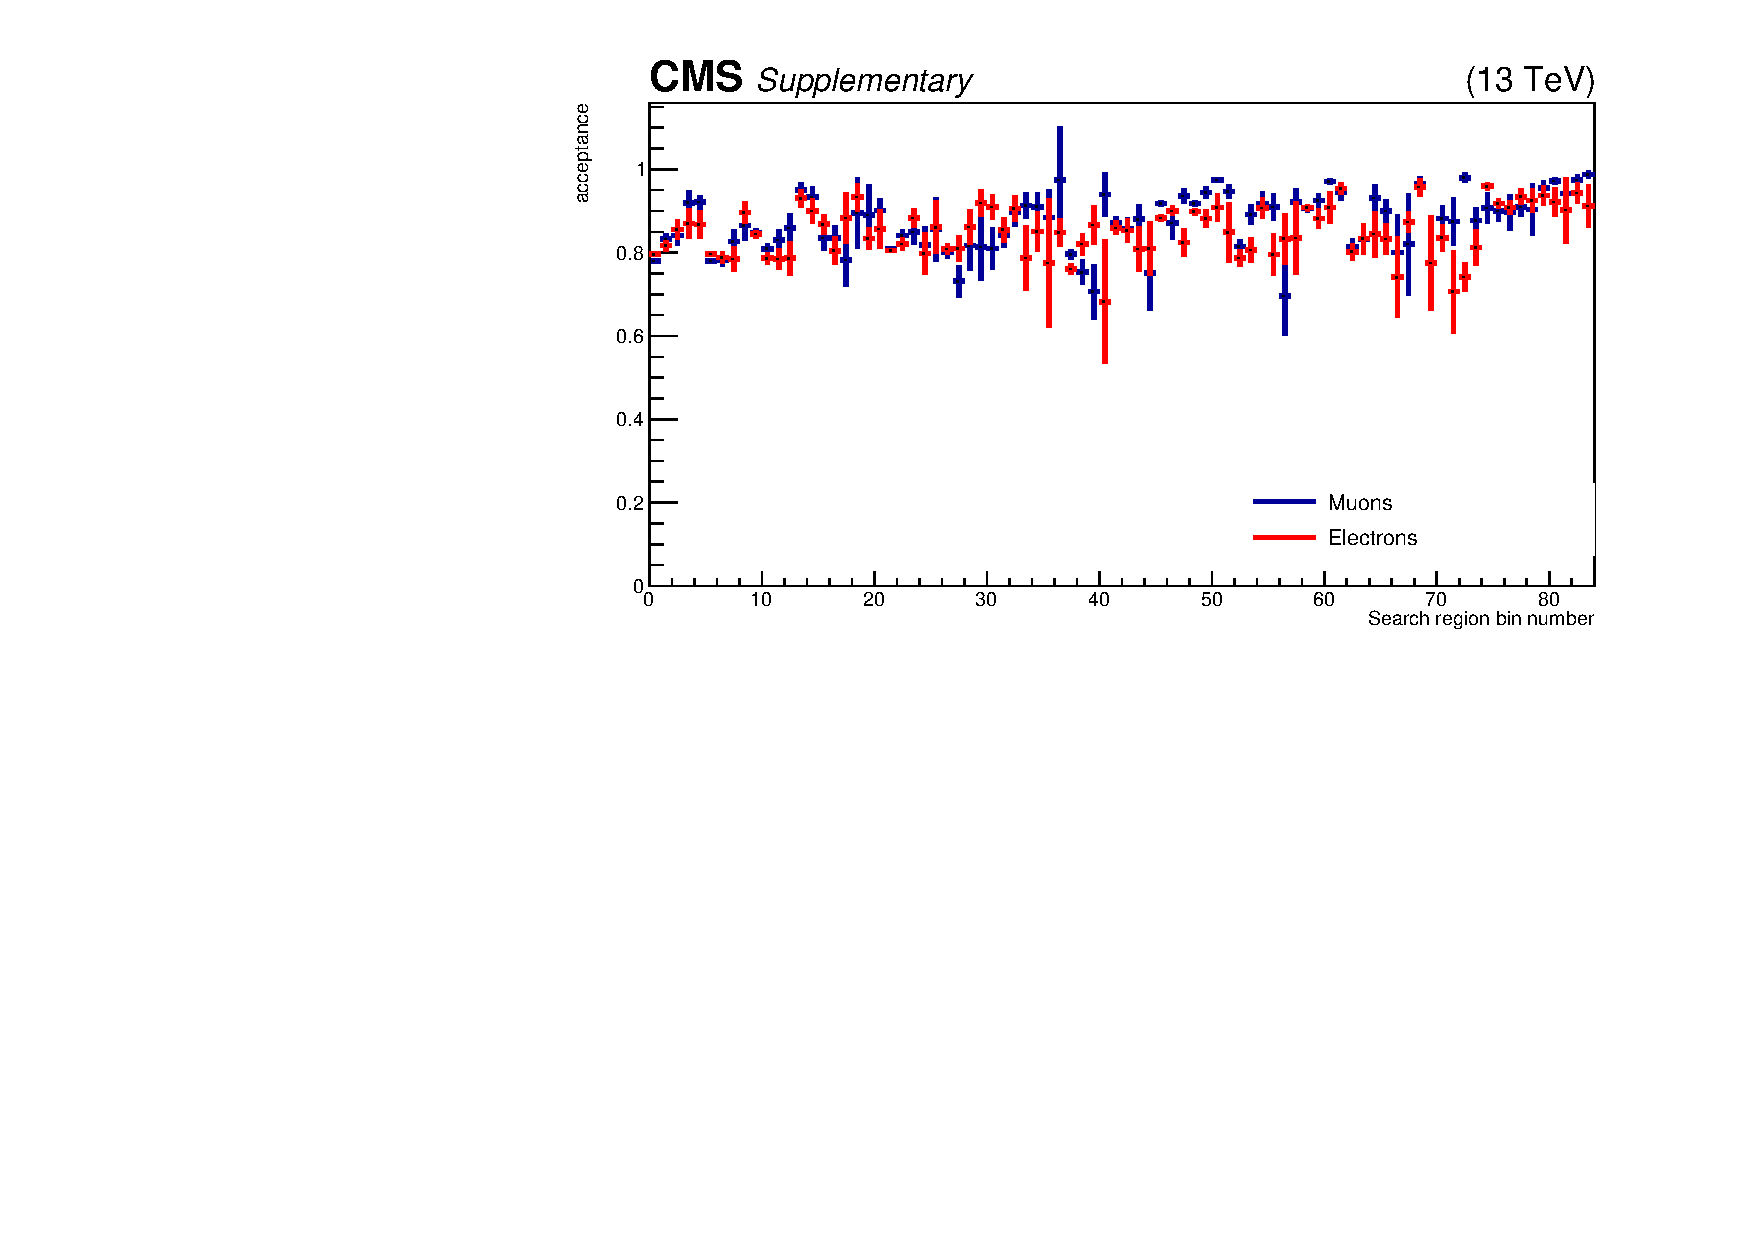
\includegraphics[width=0.9\textwidth]{sections/mc4/Backgrounds/LostLepton/figures/v2_acc_eff_84bins.pdf}%\\
\end{center}
\caption{Acceptance efficiencies for muons and electrons in each of the
search bins. Only the statistical uncertainties are shown.}
\label{fig:acceptance}
\end{figure}

The \ttbar samples include both semi-leptonic/di-leptonic inclusive samples and HT-binned samples.
The \ttbar inclusive samples have the largest weight when the samples are combined.
However, the \ttbar inclusive samples have very few events in some bins, which dramatically influences the efficiencies.
We therefore set a criterion in the acceptance and isolated track efficiency calculations that if there are less than five events in a search bin, the acceptance and isolated track efficiencies are calculated for that bin using only the HT-binned samples.

Di-lepton events may also contribute to the background if both leptons are lost.
In the muon control sample, there are di-lepton events that contribute 
when one lepton is lost while the other one is reconstructed and
identified as a muon.

If $\epsilon_{\mu}$ is the total muon efficiency 
(reco/identification times acceptance), then the 1-muon control sample contains:
\begin{itemize}
\item $\epsilon_{\mu}$ events with exactly one identified/isolated muon and 
no other lost lepton.
\item $2\epsilon_{\mu}(1-\epsilon_{\mu})$ events with one identified/isolated 
muon and one lost muon.
\item $2\epsilon_{\mu}(1-\epsilon_{e})$ events with one muon and one 
lost electron.
\end{itemize}
For these events we apply a $(1-\epsilon_{\mu})/\epsilon_{\mu}$ factor to
predict the number of events with  
lost muons and  $(1-\epsilon_{e})/\epsilon_{\mu}$ to predict the
number of lost electrons.
This leads to an overestimate in the number of lost di-leptonic events in the 
prediction by a factor of two:
\begin{itemize}
\item Two lost muons case: prediction is 
$2(1-\epsilon_{\mu})(1-\epsilon_{\mu})$, expectation 
is $(1-\epsilon_{\mu})(1-\epsilon_{\mu})$.
\item Two lost electrons case: prediction is 
$2(1-\epsilon_{e})(1-\epsilon_{e})$, 
expectation is $(1-\epsilon_{e})(1-\epsilon_{e})$.
\item One lost muon and one lost electron case: prediction is
$4(1-\epsilon_{\mu})(1-\epsilon_{e})$, 
expectation is $2(1-\epsilon_{\mu})(1-\epsilon_{e})$.
\end{itemize}
This effect is evaluated in  
simulated \ttbar, single top and W$+$jets events as the ratio between the number of events 
with one or two lost leptons over the number of events with one lost 
lepton plus twice the number of events with two lost lepton. 
Separate correction factors are applied,  
$F_{dilepton}^{\mu}$=$ (99.4\pm0.7)\% $ for muons and 
$F_{dilepton}^{e}$=$ (97.1\pm0.9)\% $ for electrons.

The purity of the electron control sample is measured in simulation and found to be $0.96\pm0.01$. The purity of the muon control sample is assumed to be 1.

Finally, the isolated track veto efficiency factor is applied in 
Eq~\ref{eq:lostleptonequation}
to get the final number of predicted lost lepton background events.
The isolated track veto efficiency is computed from simulated events 
for each search bin and shown in Fig~\ref{fig:isotrackeff}.

\begin{figure}[htbp]
\begin{center}
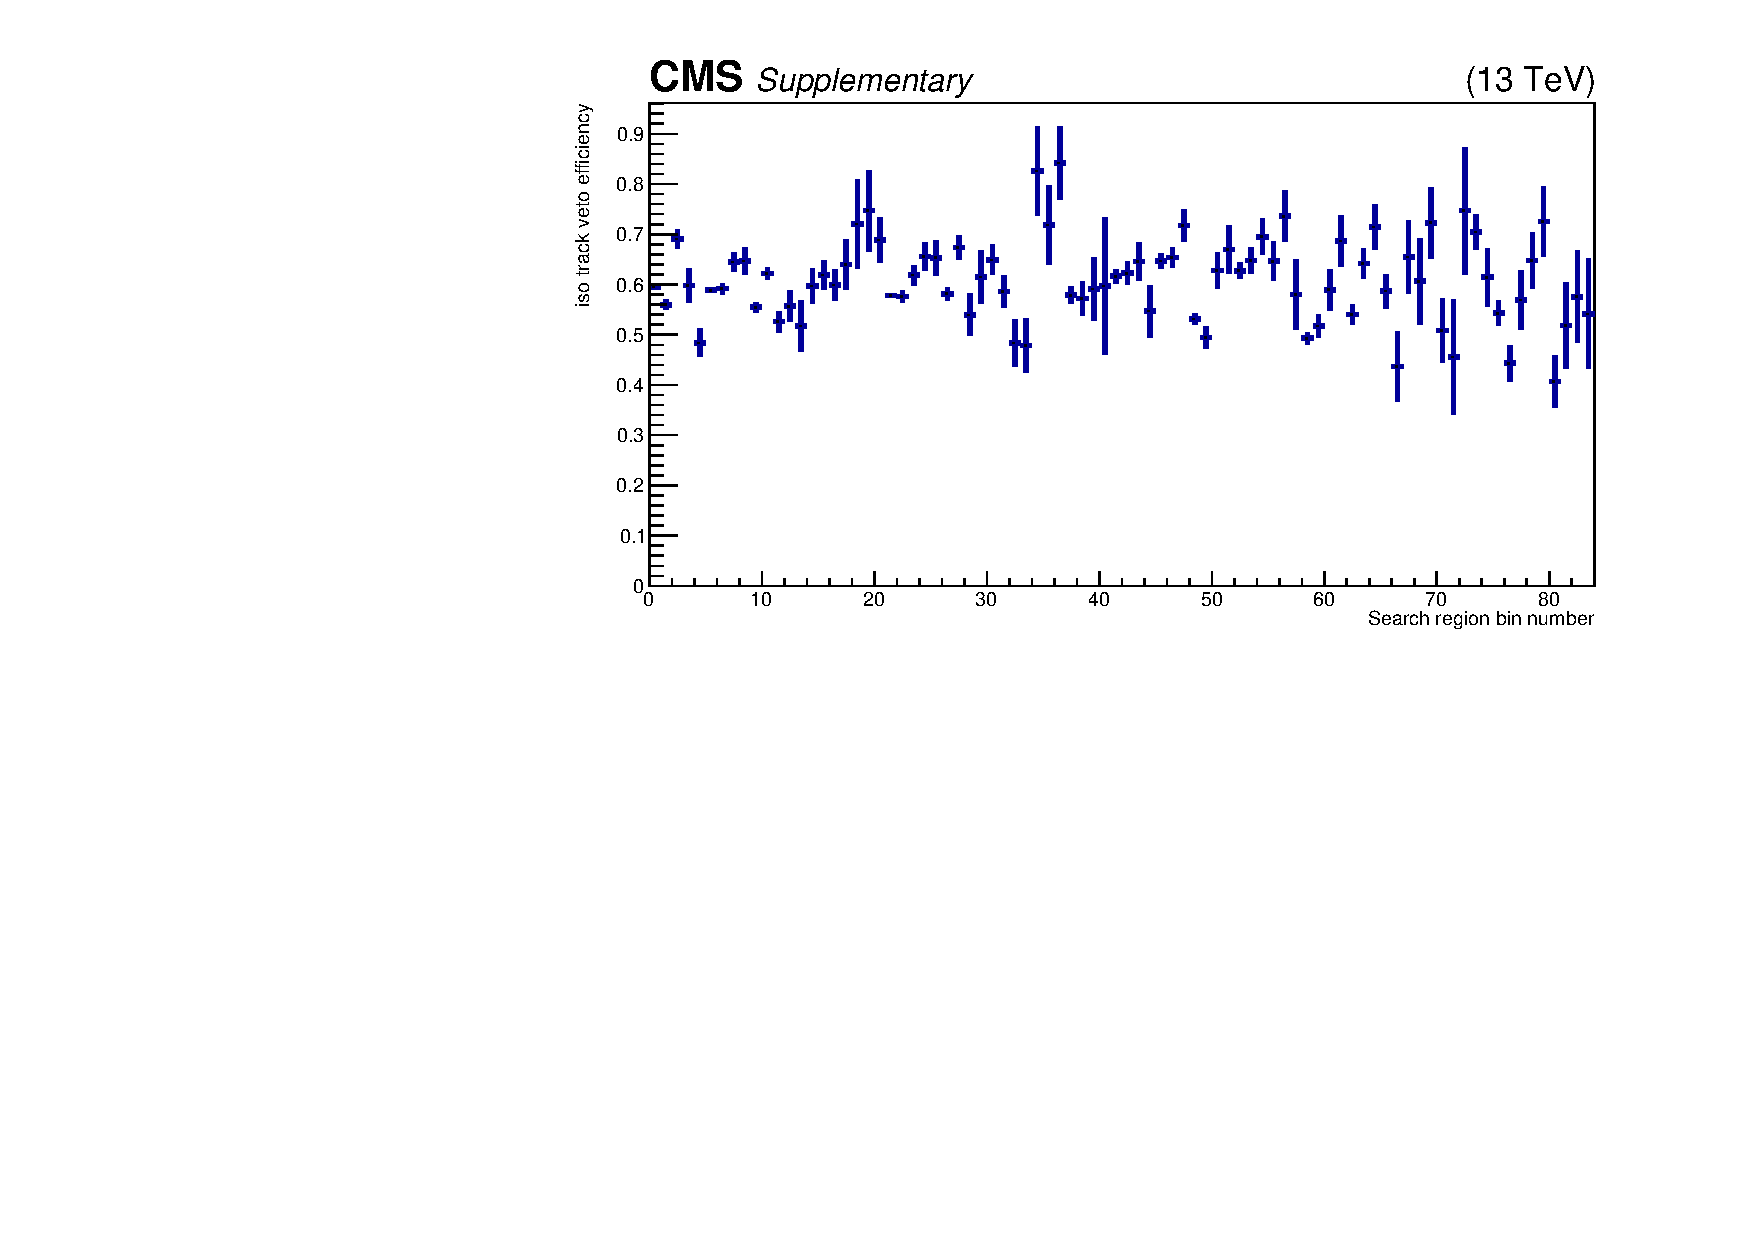
\includegraphics[width=0.9\textwidth]{sections/mc4/Backgrounds/LostLepton/figures/v2_isotrackvetoEff.pdf}%\\
\end{center}
\caption{Isolated track veto efficiencies for each search bin.}
\label{fig:isotrackeff}
\end{figure}

\paragraph{Closure Test}
Closure tests have been performed using \ttbar, single top and W$+$jets Monte Carlo samples. The prediction, i.e. the number of events obtained using the lost lepton 
method explained in the previous section is compared with the expectation, i.e. the true number of Monte Carlo simulated events with one or two lost leptons (coming from the $W$ boson produced in top quark decays). 

The results of the closure test are shown in Fig~\ref{fig:closureSBisotrk}. The expectation/prediction disagreements are propagated into the systematic uncertainty, and is the major uncertainty in the lost lepton background estimation.

\begin{figure}[htbp]
\begin{center}
\begin{tabular}{c}
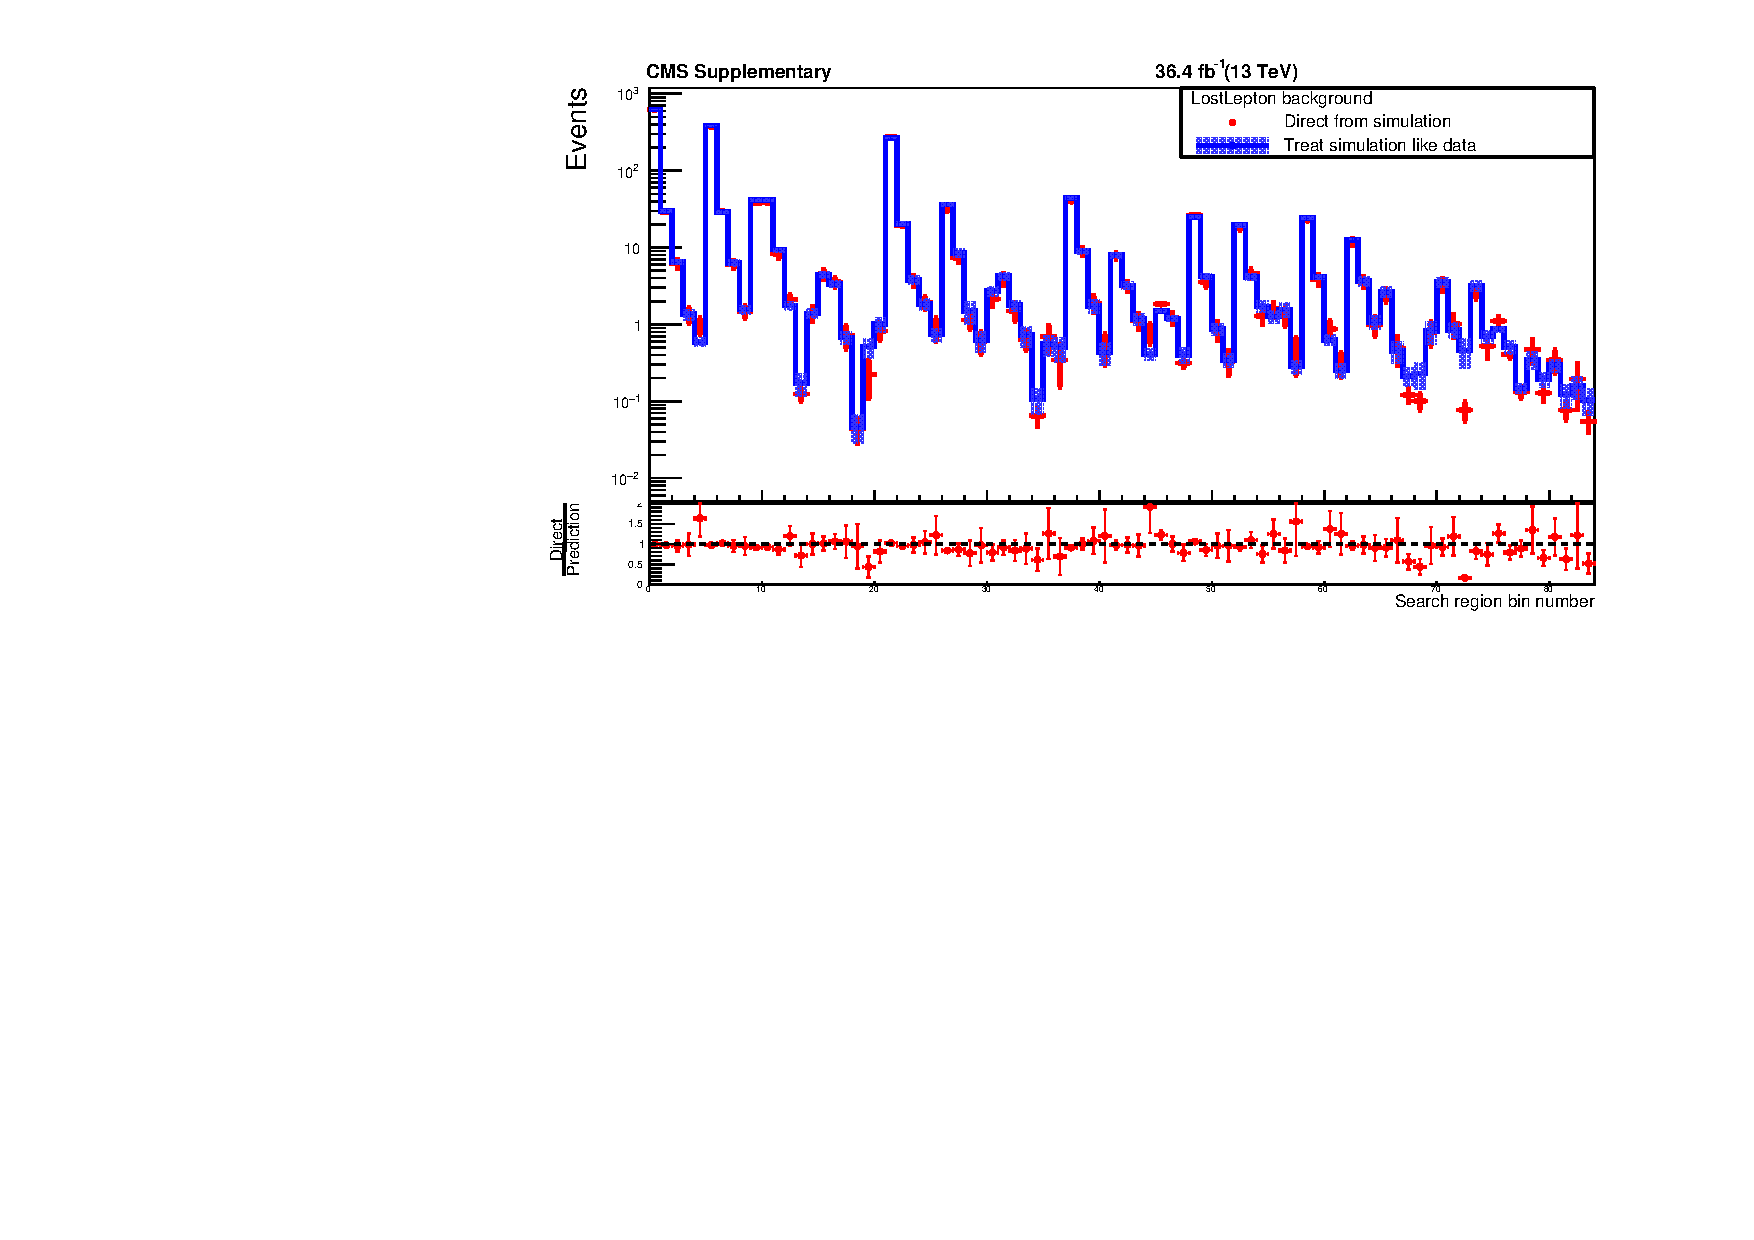
\includegraphics[width=0.85\textwidth, height=0.35\textheight]{sections/mc4/Backgrounds/LostLepton/figures/v3_closure_mu_cs.pdf}\\
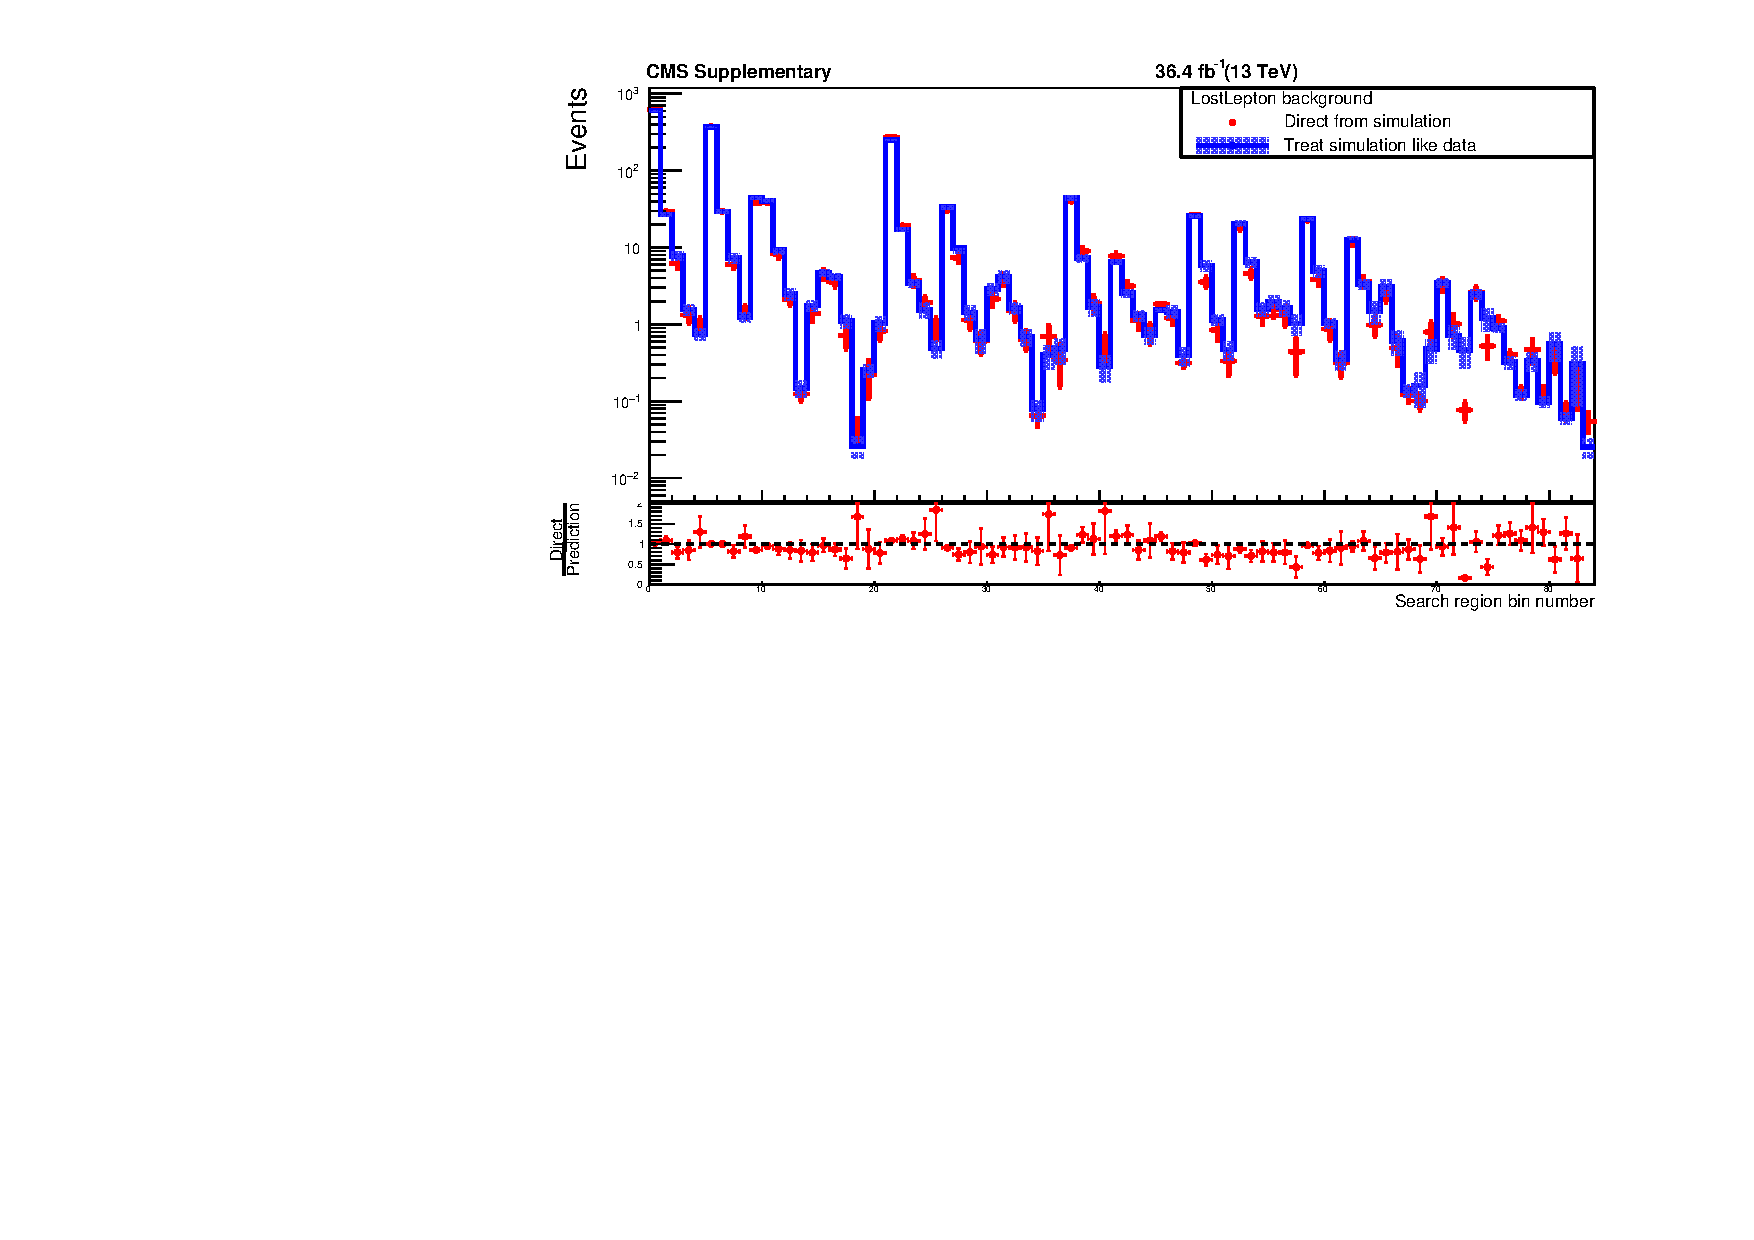
\includegraphics[width=0.85\textwidth, height=0.35\textheight]{sections/mc4/Backgrounds/LostLepton/figures/v3_closure_el_cs.pdf}
\end{tabular}
\end{center}
\caption{The lost lepton background in all the search regions of the analysis as predicted directly from \ttbar, single top and W$+$jets simulation (in red) and as predicted by applying the lost lepton background-determination procedure to simulated muon control sample (in black). The lower panel shows the ratio between the true and predicted yields. The top plot shows the prediction computed from the muon control sample. The bottom plot shows the prediction from the electron control sample.}
\label{fig:closureSBisotrk}
\end{figure}

\paragraph{Systematic uncertainties}

The following systematic uncertainties are included for the lost lepton background prediction:

\begin{itemize}
\item Lepton isolation efficiency:\\
  The muon and electron isolation efficiencies are obtained from simulated events. In order to estimate how well data and simulation agree, Tag-and-Probe efficiencies on the Z resonance from data and simulation are used, which are provided by the SUSY lepton scale-factor group. The maximum between the uncertainty obtained with the Tag-and-Probe comparing Data and simulation and the uncertainty on this value is used.
  Since no systematic bias is visible,
  no correction based on data/simulation scaling factors is introduced, and we merely take into account the systematic uncertainty obtained by propagating the SUSY lepton scale-factor group numbers.
  In addition the statistical uncertainty in the simulation efficiencies are
  propagated the same way as the Tag-and-Probe uncertainty.
  \item Lepton reconstruction/ID efficiency:\\
  The muon and electron reconstruction and ID efficiencies are obtained from simulated events. The main uncertainty here arises
  from possible differences between efficiencies obtained from data and simulation. By examining the reconstruction efficiencies as a function of the search variables it seems to be reasonable that using some inclusive efficiencies also provided by the SUSY lepton scale-factor groups are sufficient for deriving data/simulation uncertainties (same procedure as above). Furthermore, the statistical uncertainties from simulation are propagated.
\item Lepton acceptance:\\
  The uncertainty in the acceptance efficiency consists of the uncertainty
  in the parton distribution functions (PDF), the simulation renormalization/factorization scale
  and the uncertainty arising from the statistical precision of the efficiency maps.
  The PDF uncertainties are studied by varying the PDF sets used to produce the
  simulation samples, according to their uncertainties in the baseline selection.
\item Control sample purity:\\
The purity is expected to be very high ($>99\%$) so this only leads to a minor systematic uncertainty and a conservative uncertainty of 20\% on the impurity is assigned. Furthermore, the statistical uncertainties from simulation are propagated.
\item Di-lepton correction:\\
Both di-leptonic corrections are only minor compared to the remaining ones so a conservative systematic uncertainty is assigned here.
An uncertainty of 50\% is assigned on the number of di-leptonic events. Furthermore, the statistical uncertainties from simulation are propagated.
\item $M_T$ cut efficiency:\\
  The uncertainty associated with the \MT cut consists of two parts: the statistical uncertainty in the efficiency map from simulation and a systematic uncertainty. For the latter, the uncertainty in the jet energy corrections (JEC) is propagated to \MET (following the latest recommendations of the MET group) and the efficiency of the $M_T$ cut is recalculated. Following this procedure, a conservative uncertainty of 1\% is assigned as a systematic uncertainty. 
\item Isolated-track vetoes:\\
  The isolated-track vetoes lead to a reduction of about 40\%
  of the lost lepton background. Due to the size of this reduction,
  it is important to study the validity of the efficiency maps. A detailed study has been performed in the context of the RA2/b analysis~\cite{Sirunyan:2017cwe} comparing Tag-and-Probe efficiencies on the Z resonance from data and simulation. This study has shown that a systematic uncertainty of 10\% is a conservative estimate for the systematic uncertainty on the number of events removed by the isolated track veto.
\item simulation closure:\\
Furthermore, an uncertainty in the precision of the simulation closure test is assigned. Since no true non-closure is observed (see Fig~\ref{fig:closureSBisotrk}) the larger value of the non-closure or the statistical uncertainty in the non-closure is assigned for each bin. 
\end{itemize}

The source and contribution of the different components of the lost lepton method systematic uncertainties are shown in Table~\ref{tab:systematics}.

\begin{table}[htbp]
\fontsize{10 pt}{1.2 em}
\caption{Source and contribution of the different components of the lost lepton method systematic uncertainties.} 
\begin{center}
\begin{tabular}{|c|c|c|c|}
\hline
Source & Note & \specialcell{Electron \\ control sample} & \specialcell{Muon \\ control sample} \\
\hline
Muon Iso 			& \specialcell{Data-MC correction \\ from tag and probe} & 1\% to 3\% & 1\% to 4\% \\
\hline
Elec Iso 			& \specialcell{Data-MC correction \\ from tag and probe} & 4\% to 8\% & 2\% to 5\% \\
\hline
Muon ID 			& \specialcell{Data-MC correction \\ from tag and probe} & 2\% to 7\% & 4\% to 11\% \\
\hline
Elec ID 			& \specialcell{Data-MC correction \\ from tag and probe} & 6\% to 11\% & 2\% to 8\% \\
\hline
Acceptance    & \specialcell{PDF and MC \\ scale variation} & 4\% to 97\% & 4\% to 97\% \\ 
\hline
\specialcell{Other SM \\ contribution}  & \specialcell{20\% uncertainty on the purity} & 0\% & 0\% \\
\hline
\specialcell{Di-Muon \\ Correction}     & \specialcell{Statistical uncertainty + 50\%} & 0\% & 0\% \\
\hline
\specialcell{Di-Electron \\ Correction} & \specialcell{Statistical uncertainty + 50\%} & 1\% & 1\% \\
\hline
\specialcell{Transverse \\ Mass Cut}    & \specialcell{Variation of \MET energy scale} & 0\% & 0\% \\
\hline
\specialcell{Isolated \\ track veto}    & \specialcell{Data-MC correction \\ on isolated track \\ veto efficiencies} & 10\% & 10\% \\
\hline
Closure & \specialcell{Non-closure and \\ statistical precision \\ of the closure} & 2\% to 104\% & 2\% to 86\% \\
\hline
Total	& & 13\% to 143\% & 12\% to 131\% \\
\hline
\end{tabular}
\end{center}
\label{tab:systematics}
\end{table}

\paragraph{Lost Lepton background prediction}

The lost lepton method is applied to data event samples (collected with the search triggers) corresponding to an integrated luminosity of $35.9$~fb$^{-1}$. The final predictions for all search bins are shown in Figs~\ref{fig:LostLeptonResult_mu} and \ref{fig:LostLeptonResult_el} (red points) and listed in Tables~\ref{tab:LLpredmu1}-\ref{tab:LLpredel3} for both the muon and electron channels.

Applying the procedure indicated by Eq.~\ref{eq:lostleptonequation}, each event in the control sample is weighted by the various efficiencies. 
A few bins have zero predicted events. In that case the statistical uncertainty is computed as the upper bound of the statistical uncertainty on 0 given by the Garwood interval (1.8) multiplied by the average translation factor to go from a raw number of events to the prediction. This Poisson uncertainty is treated in the Higgs combination tool using a gamma function~\cite{HiggsCombine,cms-note-2011-005}.

\begin{figure}[hptb]
\begin{center}
\begin{tabular}{c}
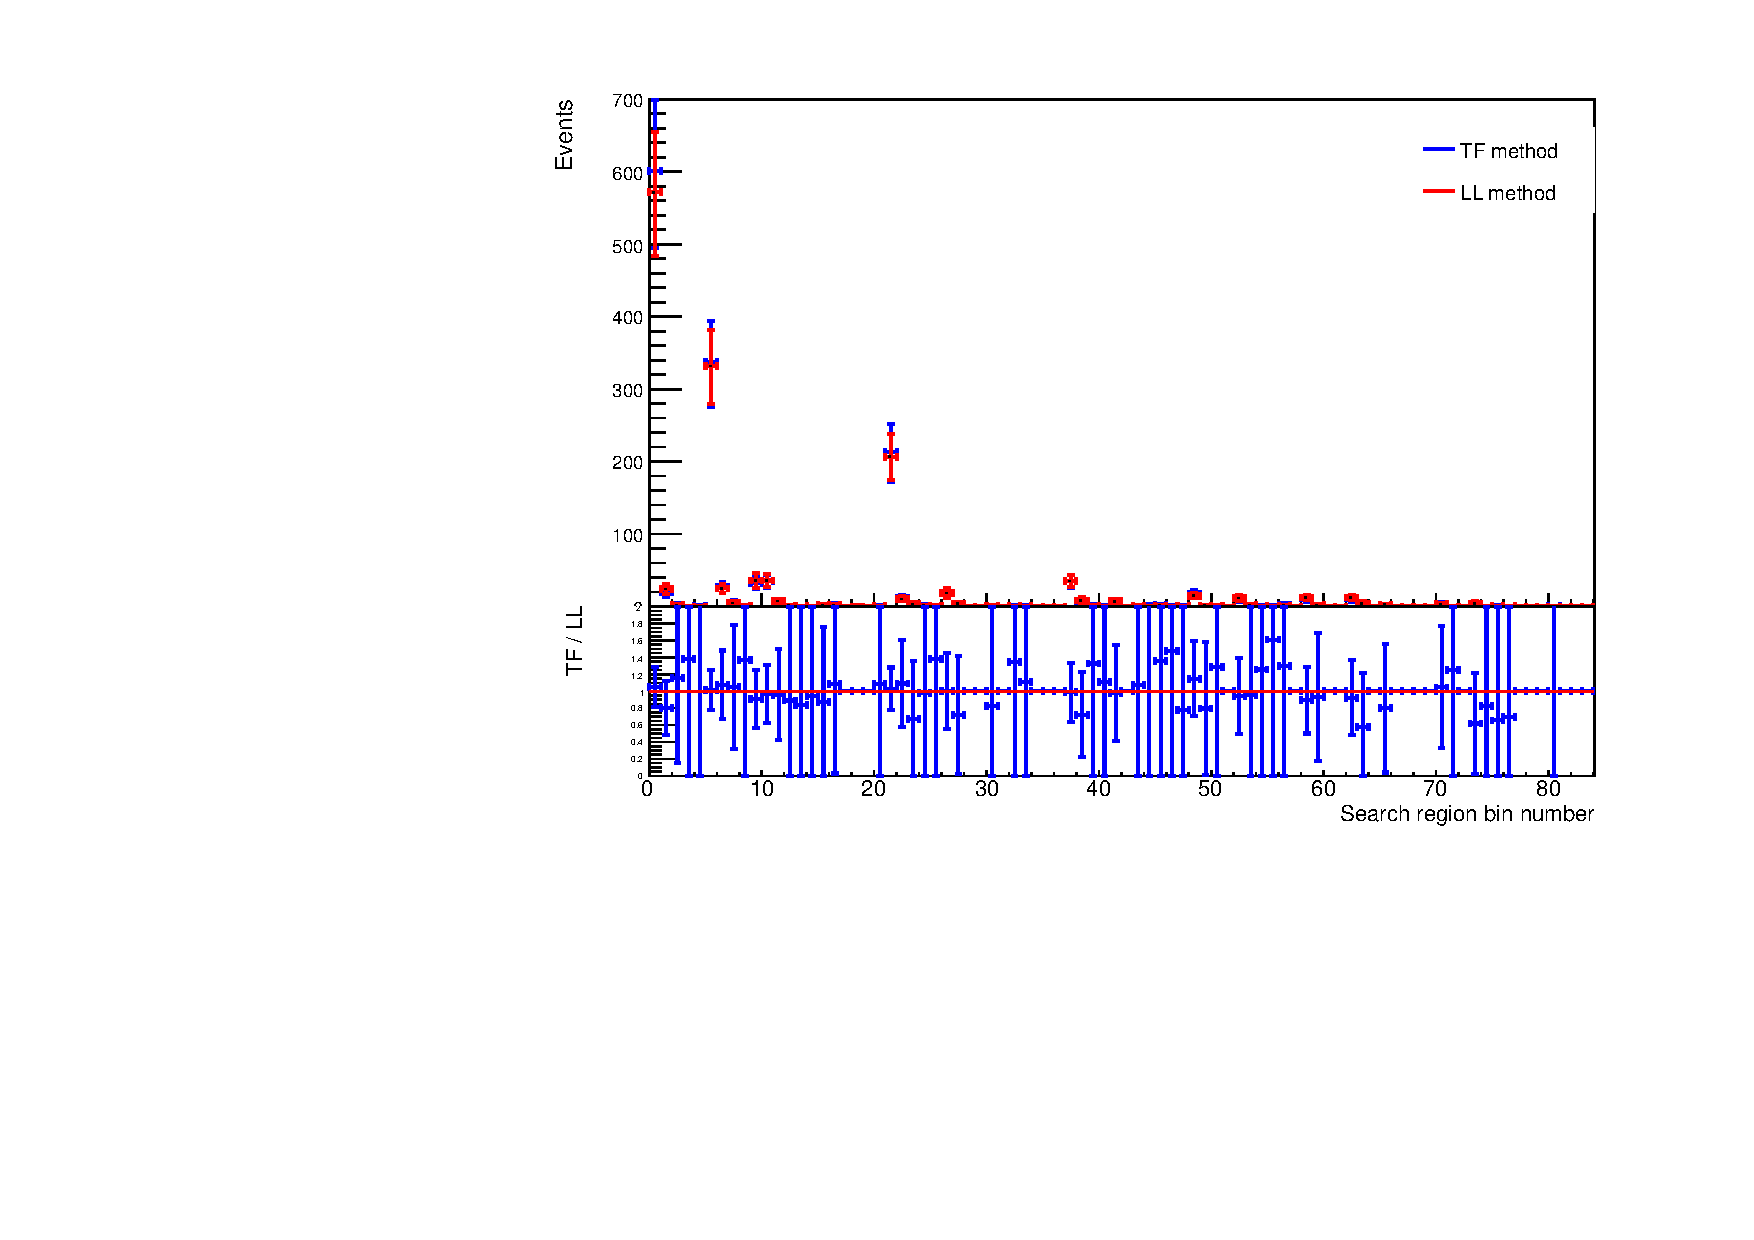
\includegraphics[width=0.50\textwidth]{sections/mc4/Backgrounds/LostLepton/figures/v4_DataCardCampare_0_700_mu_cs.pdf}\\
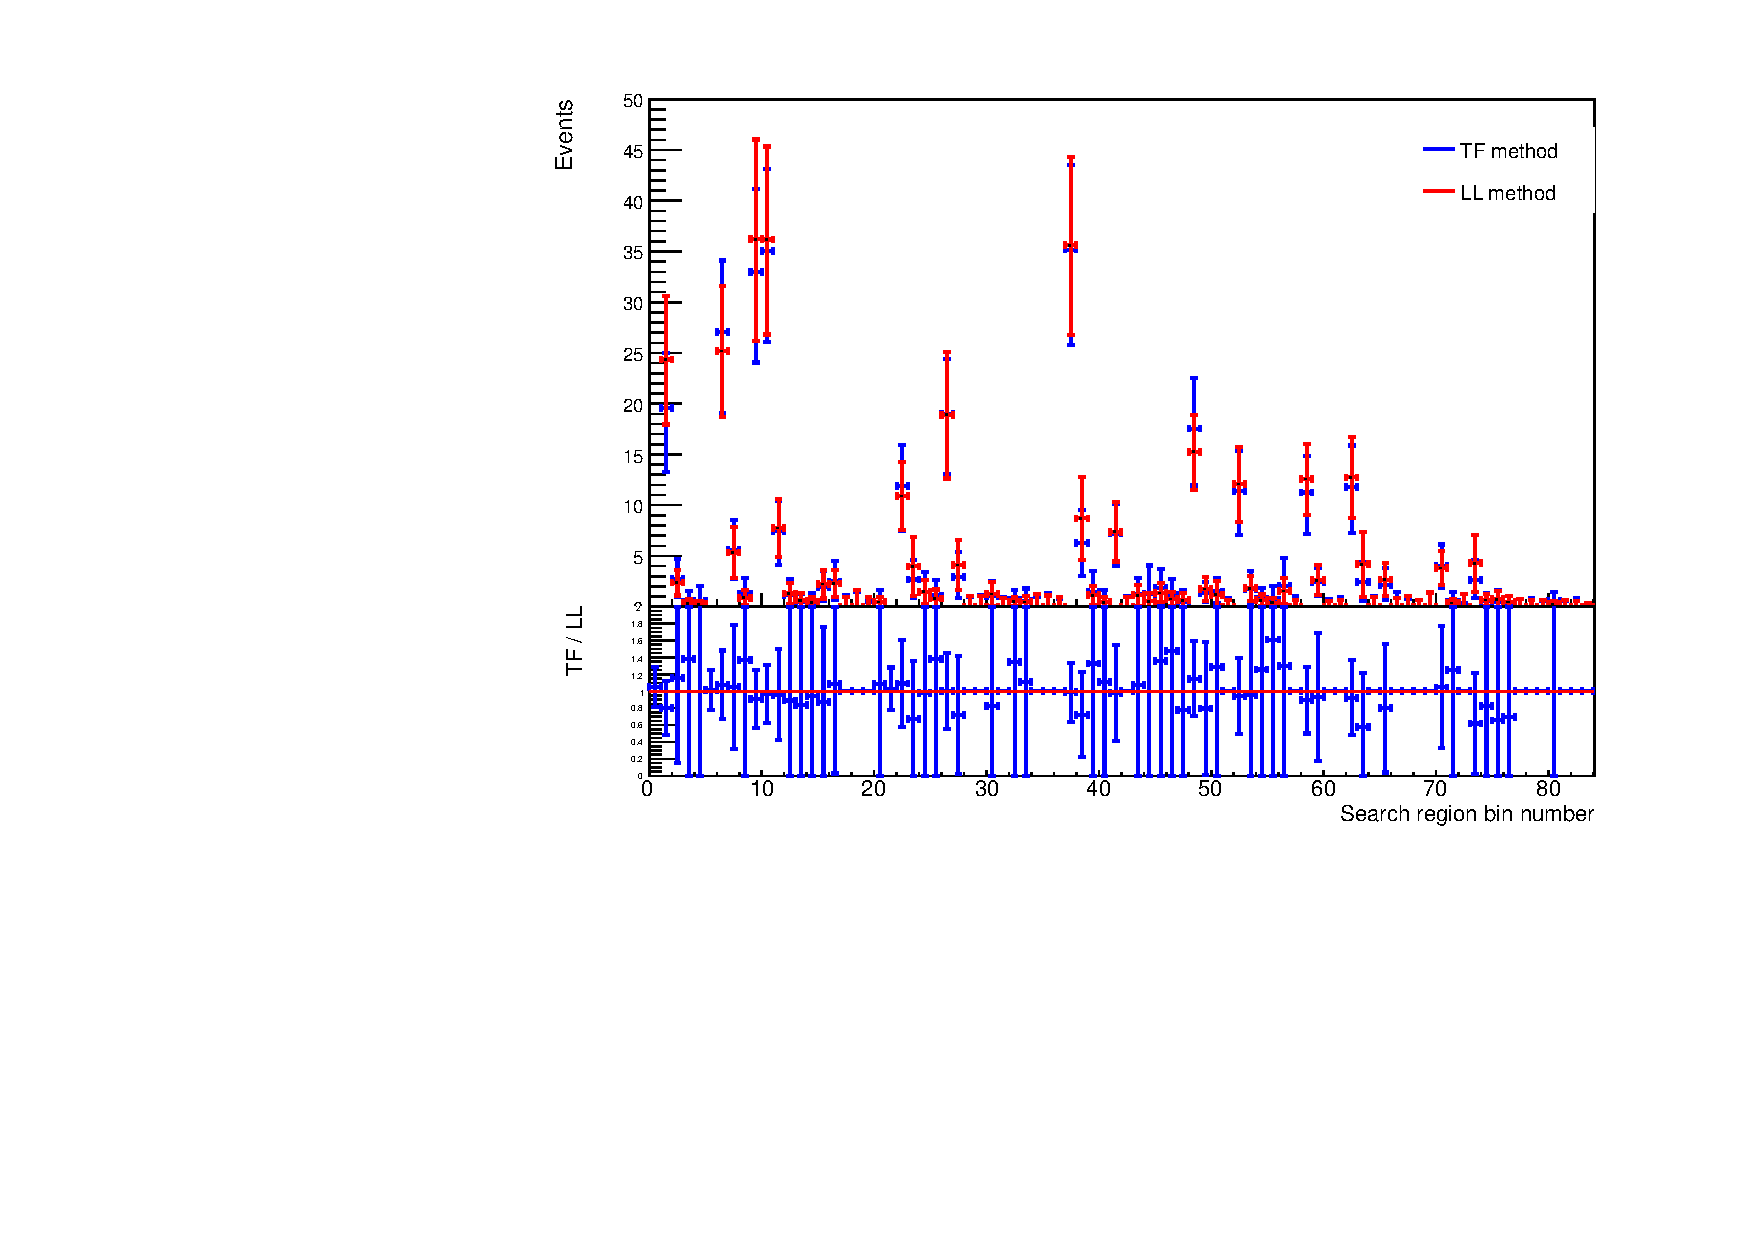
\includegraphics[width=0.40\textwidth]{sections/mc4/Backgrounds/LostLepton/figures/v4_DataCardCampare_0_50_mu_cs.pdf}
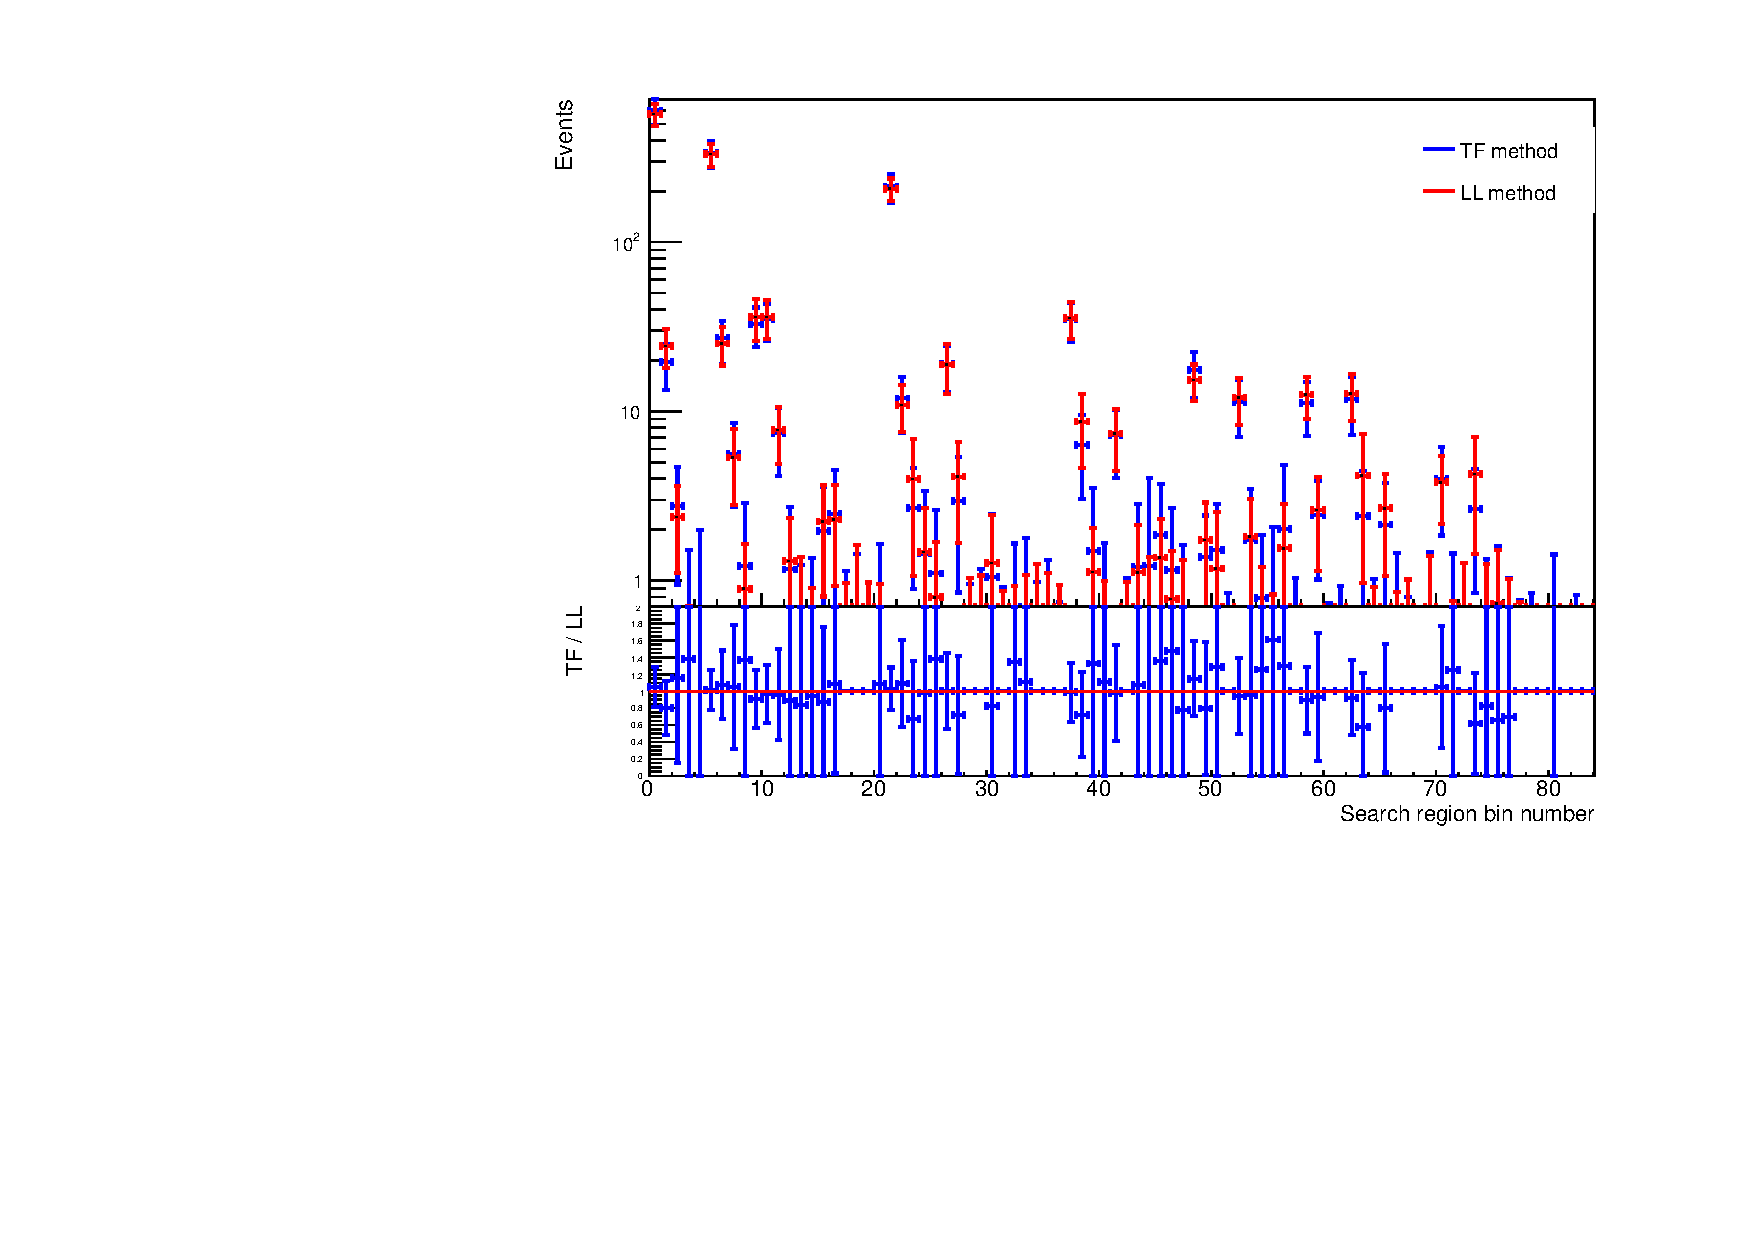
\includegraphics[width=0.40\textwidth]{sections/mc4/Backgrounds/LostLepton/figures/v4_DataCardCampare_0_700_mu_cs_log.pdf}
\end{tabular}
\end{center}
\caption{Lost lepton background predictions on muon control sample, in red. The blue points are the results obtained with the average TF method. The uncertainties include both the statistical and systematic uncertainties. Bottom left plot is a zoom of the top plot and the bottom right plot is log scale.}
\label{fig:LostLeptonResult_mu}
\end{figure}

\begin{figure}[hptb]
\begin{center}
\begin{tabular}{c}
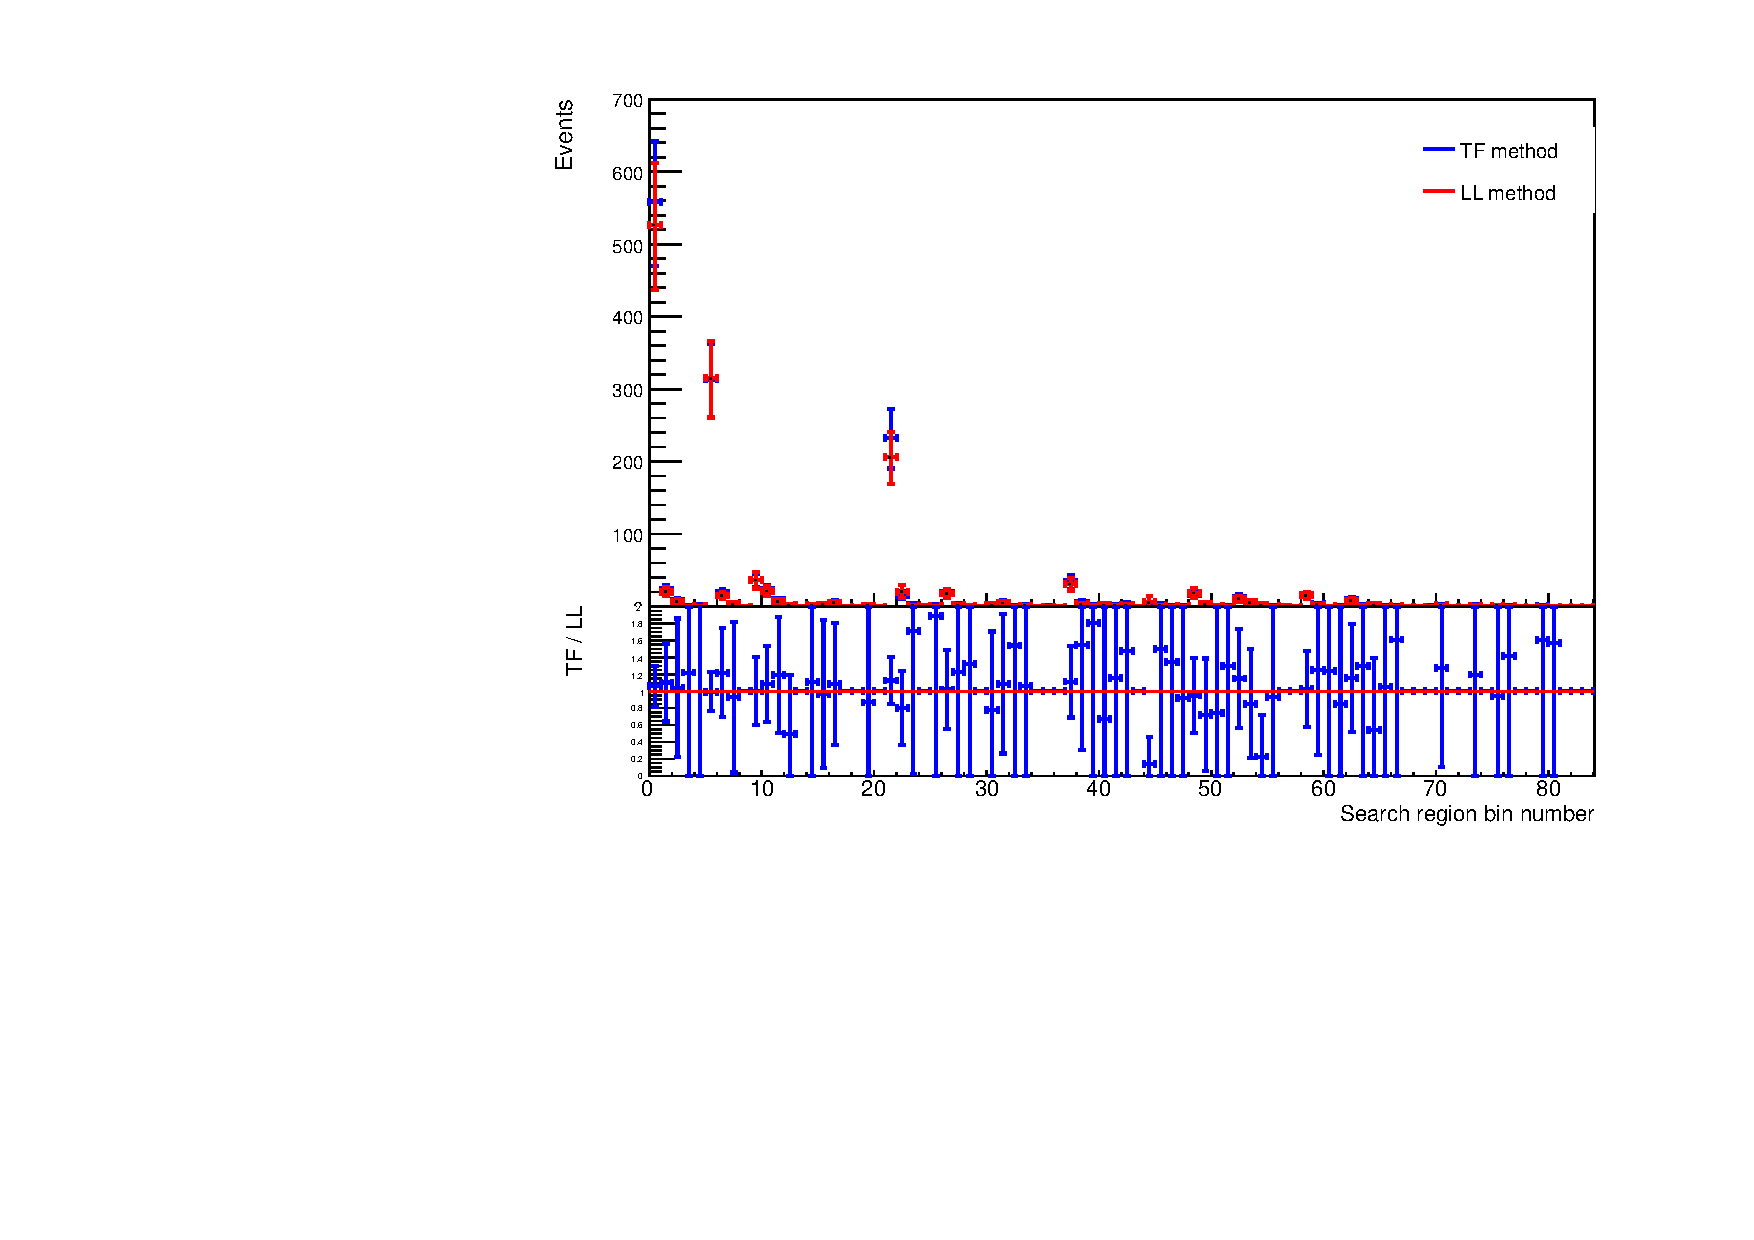
\includegraphics[width=0.50\textwidth]{sections/mc4/Backgrounds/LostLepton/figures/v4_DataCardCampare_0_700_el_cs.pdf}\\
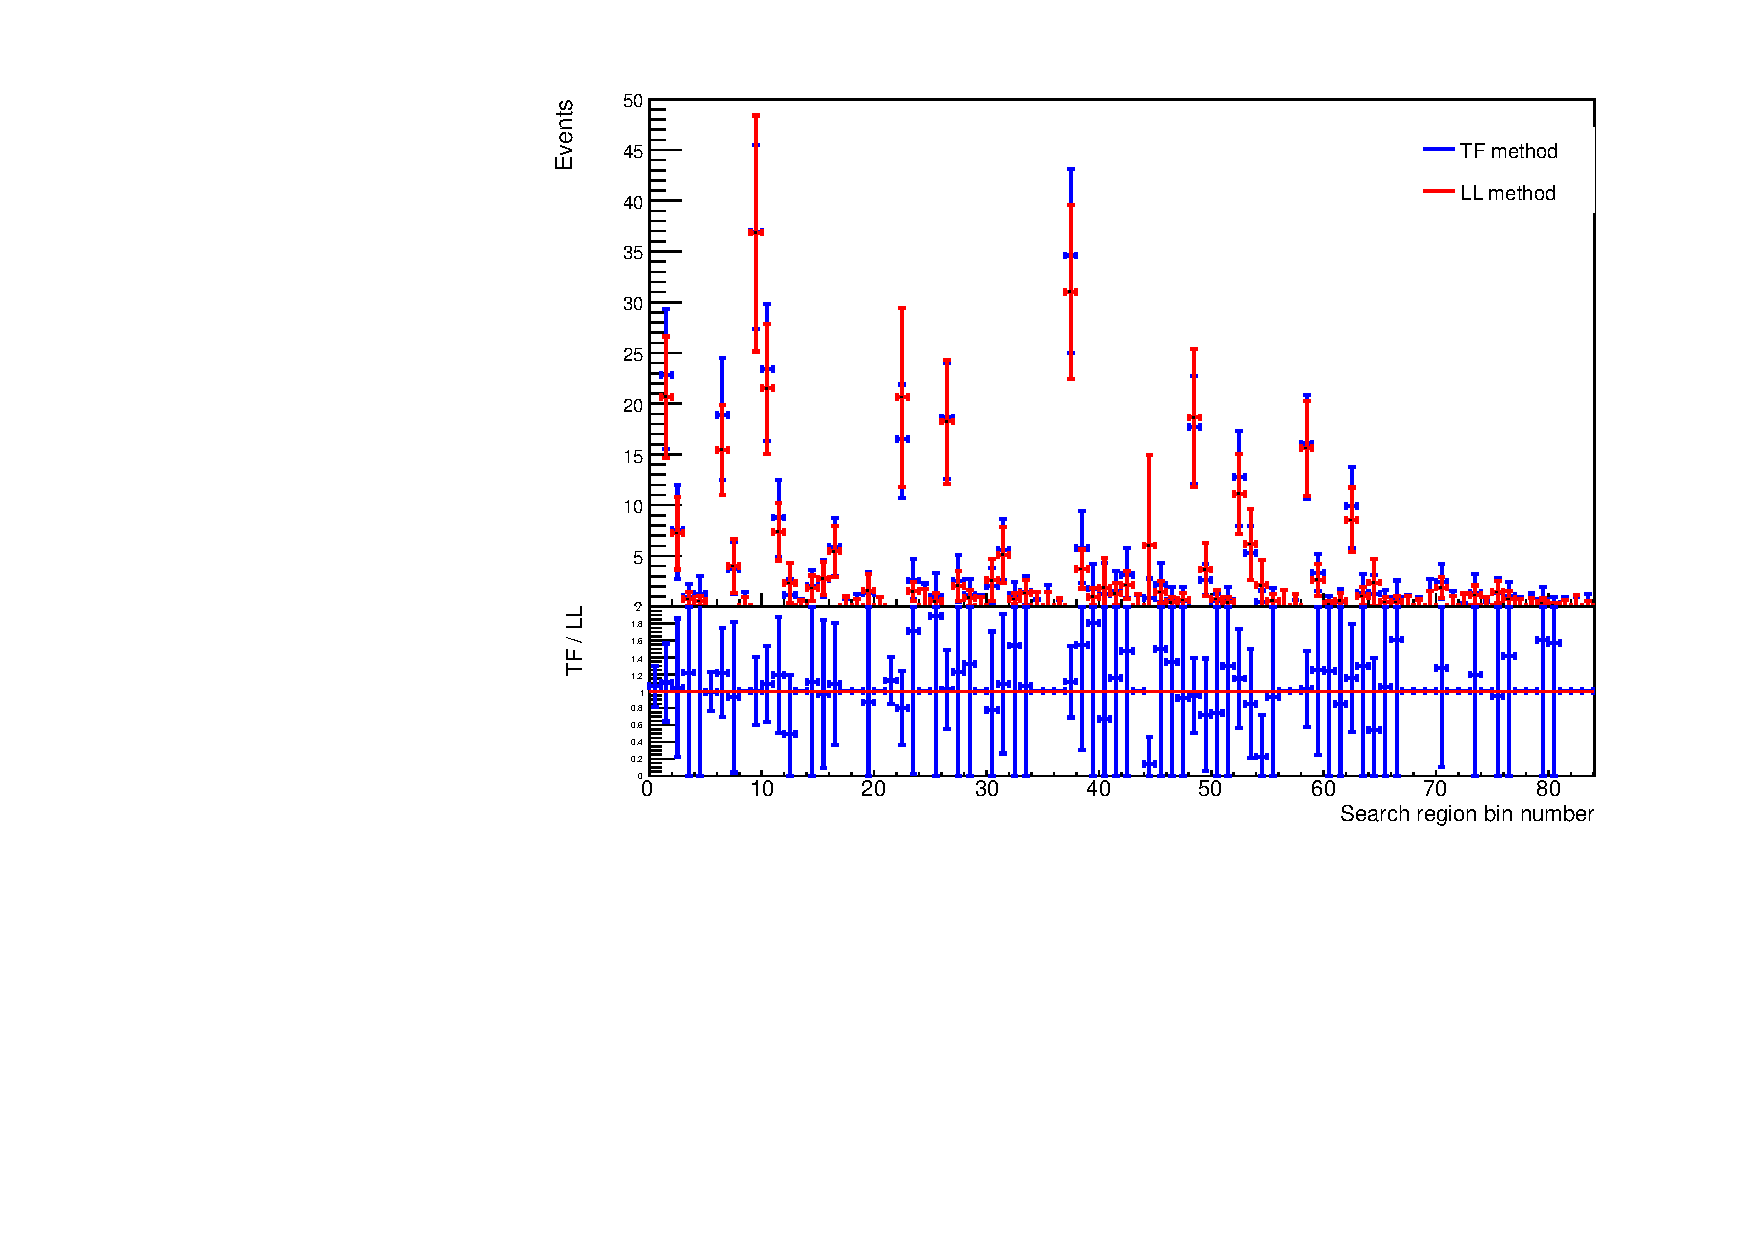
\includegraphics[width=0.40\textwidth]{sections/mc4/Backgrounds/LostLepton/figures/v4_DataCardCampare_0_50_el_cs.pdf}
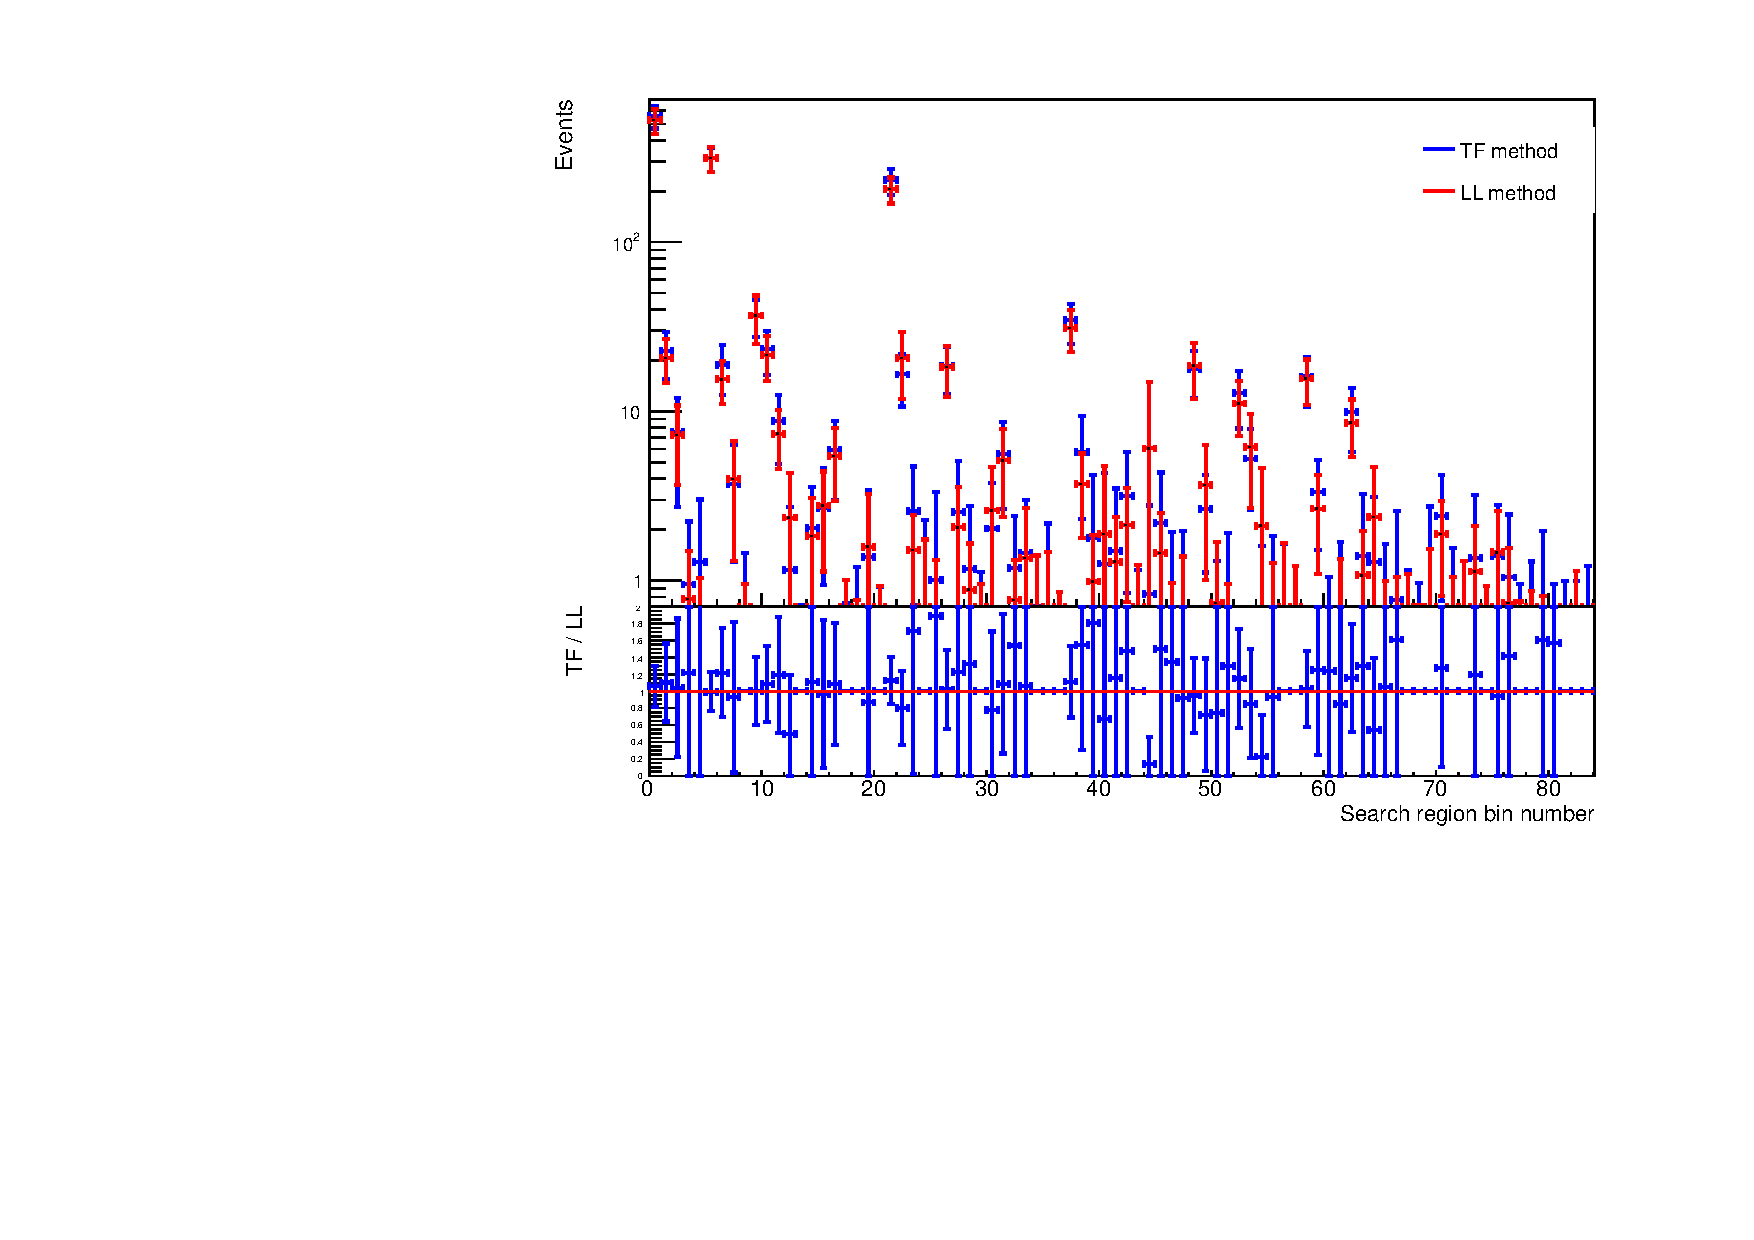
\includegraphics[width=0.40\textwidth]{sections/mc4/Backgrounds/LostLepton/figures/v4_DataCardCampare_0_700_el_cs_log.pdf}
\end{tabular}
\end{center}
\caption{Lost lepton background predictions on electron control sample, in red. The blue points are the results obtained with the average TF method. The uncertainties include both the statistical and systematic uncertainties. Bottom left plot is a zoom of the top plot and the bottom right plot is log scale.}
\label{fig:LostLeptonResult_el}
\end{figure}

\begin{table}[htbp]
\fontsize{10 pt}{1.2 em}
\selectfont
\begin{centering}
\caption{\label{tab:LLpredmu1} Predicted lost lepton background yield from the muon control sample with statistical and systematic uncertainties for a $35.9$~fb$^{-1}$ sample.}
\hspace*{-4ex}
\begin{tabular}{|c|c|c|c|c||c|}
\hline
Search Bin & \ntops & \nbjets & \MTTwo [GeV] & \MET [GeV] & Lost Lepton Prediction\\
\hline
0 &               1 &               1 &         200-300 &         250-400 & 571.615 $^{+21.270}_{-21.237}$ $^{+80.824}_{-85.452}$ \\ 
\hline
1 &               1 &               1 &         200-300 &         400-500 & 24.355 $^{+4.936}_{-4.837}$ $^{+4.015}_{-4.201}$ \\ 
\hline
2 &               1 &               1 &         200-300 &         500-600 & 2.376 $^{+1.520}_{-1.070}$ $^{+0.669}_{-0.682}$ \\ 
\hline
3 &               1 &               1 &         200-300 &         600-750 & 0.331 $^{+0.824}_{-0.331}$ $^{+0.182}_{-0.183}$ \\ 
\hline
4 &               1 &               1 &         200-550 &            750+ & 0.231 $^{+0.607}_{-0.231}$ $^{+0.150}_{-0.150}$ \\ 
\hline
5 &               1 &               1 &         300-400 &         250-400 & 332.123 $^{+16.111}_{-16.070}$ $^{+47.094}_{-49.965}$ \\ 
\hline
6 &               1 &               1 &         300-400 &         400-500 & 25.202 $^{+4.961}_{-4.816}$ $^{+4.242}_{-4.427}$ \\ 
\hline
7 &               1 &               1 &         300-400 &         500-600 & 5.341 $^{+2.178}_{-1.815}$ $^{+1.749}_{-1.773}$ \\ 
\hline
8 &               1 &               1 &         300-400 &         600-750 & 0.894 $^{+1.127}_{-0.645}$ $^{+0.369}_{-0.372}$ \\ 
\hline
9 &               1 &               1 &         400-550 &         250-400 & 36.205 $^{+5.030}_{-4.960}$ $^{+8.485}_{-8.724}$ \\ 
\hline
10 &               1 &               1 &         400-550 &         400-500 & 36.177 $^{+5.448}_{-5.329}$ $^{+7.466}_{-7.691}$ \\ 
\hline
11 &               1 &               1 &         400-550 &         500-600 & 7.748 $^{+2.303}_{-2.102}$ $^{+1.895}_{-1.937}$ \\ 
\hline
12 &               1 &               1 &         400-550 &         600-750 & 1.306 $^{+1.277}_{-0.924}$ $^{+0.449}_{-0.453}$ \\ 
\hline
13 &               1 &               1 &         550-750 &         250-400 & 0.609 $^{+0.681}_{-0.445}$ $^{+0.632}_{-0.633}$ \\ 
\hline
14 &               1 &               1 &         550-750 &         400-500 & 0.432 $^{+0.756}_{-0.432}$ $^{+0.185}_{-0.187}$ \\ 
\hline
15 &               1 &               1 &         550-750 &         500-600 & 2.232 $^{+1.523}_{-1.234}$ $^{+0.705}_{-0.719}$ \\ 
\hline
16 &               1 &               1 &         550-750 &         600-750 & 2.293 $^{+1.551}_{-1.177}$ $^{+0.674}_{-0.688}$ \\ 
\hline
17 &               1 &               1 &         550-750 &            750+ & 0.000 $^{+0.990}_{-0.000}$ $^{+0.000}_{-0.000}$ \\ 
\hline
18 &               1 &               1 &            750+ &         250-600 & 0.000 $^{+1.661}_{-0.000}$ $^{+0.000}_{-0.000}$ \\ 
\hline
19 &               1 &               1 &            750+ &         600-750 & 0.000 $^{+0.992}_{-0.000}$ $^{+0.000}_{-0.000}$ \\ 
\hline
20 &               1 &               1 &            750+ &            750+ & 0.446 $^{+1.055}_{-0.446}$ $^{+0.243}_{-0.244}$ \\ 
\hline
21 &               1 &               2 &         200-350 &         250-400 & 207.008 $^{+12.950}_{-12.904}$ $^{+28.139}_{-29.923}$ \\ 
\hline
22 &               1 &               2 &         200-350 &         400-500 & 10.922 $^{+2.757}_{-2.558}$ $^{+2.101}_{-2.173}$ \\ 
\hline
23 &               1 &               2 &         200-350 &         500-600 & 3.971 $^{+2.797}_{-2.627}$ $^{+1.238}_{-1.259}$ \\ 
\hline
24 &               1 &               2 &         200-350 &         600-750 & 1.471 $^{+1.617}_{-1.043}$ $^{+0.595}_{-0.598}$ \\ 
\hline
25 &               1 &               2 &         200-650 &            750+ & 0.796 $^{+1.127}_{-0.563}$ $^{+0.694}_{-0.700}$ \\ 
\hline
26 &               1 &               2 &         350-450 &         250-400 & 18.915 $^{+3.488}_{-3.308}$ $^{+5.244}_{-5.348}$ \\ 
\hline
27 &               1 &               2 &         350-450 &         400-500 & 4.115 $^{+2.637}_{-2.118}$ $^{+1.215}_{-1.231}$ \\ 
\hline
28 &               1 &               2 &         350-450 &         500-600 & 0.000 $^{+1.057}_{-0.000}$ $^{+0.000}_{-0.000}$ \\ 
\hline
29 &               1 &               2 &         350-450 &         600-750 & 0.000 $^{+1.090}_{-0.000}$ $^{+0.000}_{-0.000}$ \\ 
\hline
30 &               1 &               2 &         450-650 &         250-400 & 1.269 $^{+1.452}_{-0.926}$ $^{+0.692}_{-0.695}$ \\ 
\hline
31 &               1 &               2 &         450-650 &         400-500 & 0.000 $^{+0.884}_{-0.000}$ $^{+0.000}_{-0.000}$ \\ 
\hline
32 &               1 &               2 &         450-650 &         500-600 & 0.519 $^{+0.701}_{-0.370}$ $^{+0.184}_{-0.185}$ \\ 
\hline
33 &               1 &               2 &         450-650 &         600-750 & 0.482 $^{+1.016}_{-0.482}$ $^{+0.352}_{-0.353}$ \\ 
\hline
34 &               1 &               2 &            650+ &         250-600 & 0.000 $^{+1.282}_{-0.000}$ $^{+0.000}_{-0.000}$ \\ 
\hline
35 &               1 &               2 &            650+ &         600-750 & 0.000 $^{+1.123}_{-0.000}$ $^{+0.000}_{-0.000}$ \\ 
\hline
36 &               1 &               2 &            650+ &            750+ & 0.000 $^{+0.953}_{-0.000}$ $^{+0.000}_{-0.000}$ \\ 
\hline
\end{tabular}
\par\end{centering}
\end{table}

\begin{table}[htbp]
\fontsize{10 pt}{1.2 em}
\selectfont
\begin{centering}
\caption{\label{tab:LLpredmu2} Predicted lost lepton background yield from the muon control sample with statistical and systematic uncertainties for a $35.9$~fb$^{-1}$ sample.}
\hspace*{-4ex}
\begin{tabular}{|c|c|c|c|c||c|}
\hline
37 &               1 &              3+ &        300-1000 &         250-350 & 35.608 $^{+5.692}_{-5.569}$ $^{+6.655}_{-6.875}$ \\ 
\hline
38 &               1 &              3+ &        300-1000 &         350-450 & 8.699 $^{+3.703}_{-3.514}$ $^{+1.994}_{-2.035}$ \\ 
\hline
39 &               1 &              3+ &        300-1000 &         450-550 & 1.120 $^{+1.490}_{-0.792}$ $^{+0.472}_{-0.476}$ \\ 
\hline
40 &               1 &              3+ &        300-1000 &            550+ & 0.440 $^{+0.908}_{-0.440}$ $^{+0.330}_{-0.331}$ \\ 
\hline
41 &               1 &              3+ &       1000-1500 &         250-350 & 7.396 $^{+2.601}_{-2.400}$ $^{+1.654}_{-1.697}$ \\ 
\hline
42 &               1 &              3+ &       1000-1500 &         350-450 & 0.000 $^{+0.992}_{-0.000}$ $^{+0.000}_{-0.000}$ \\ 
\hline
43 &               1 &              3+ &       1000-1500 &         450-550 & 1.118 $^{+1.319}_{-0.827}$ $^{+0.589}_{-0.592}$ \\ 
\hline
44 &               1 &              3+ &       1000-1500 &            550+ & 0.520 $^{+1.291}_{-0.520}$ $^{+0.674}_{-0.674}$ \\ 
\hline
45 &               1 &              3+ &           1500+ &         250-350 & 1.366 $^{+1.192}_{-0.818}$ $^{+0.459}_{-0.467}$ \\ 
\hline
46 &               1 &              3+ &           1500+ &         350-550 & 0.777 $^{+1.127}_{-0.553}$ $^{+0.449}_{-0.451}$ \\ 
\hline
47 &               1 &              3+ &           1500+ &            550+ & 0.626 $^{+1.199}_{-0.626}$ $^{+0.321}_{-0.325}$ \\ 
\hline
\end{tabular}
\par\end{centering}
\end{table}

\begin{table}[htbp]
\fontsize{10 pt}{1.2 em}
\selectfont
\begin{centering}
\caption{\label{tab:LLpredmu3} Predicted lost lepton background yield from the muon control sample with statistical and systematic uncertainties for a $35.9$~fb$^{-1}$ sample.}
\hspace*{-4ex}
\begin{tabular}{|c|c|c|c|c||c|}
\hline
Search Bin & \ntops & \nbjets & \MTTwo [GeV] & \MET [GeV] & Lost Lepton Prediction\\
\hline
48 &               2 &               1 &         200-300 &         250-350 & 15.278 $^{+2.515}_{-2.443}$ $^{+2.699}_{-2.889}$ \\ 
\hline
49 &               2 &               1 &         200-300 &         350-450 & 1.733 $^{+1.132}_{-0.989}$ $^{+0.601}_{-0.617}$ \\ 
\hline
50 &               2 &               1 &         200-300 &         450-600 & 1.176 $^{+0.884}_{-0.649}$ $^{+1.195}_{-1.197}$ \\ 
\hline
51 &               2 &               1 &         200-450 &            600+ & 0.000 $^{+0.705}_{-0.000}$ $^{+0.000}_{-0.000}$ \\ 
\hline
52 &               2 &               1 &         300-450 &         250-350 & 12.074 $^{+3.125}_{-2.893}$ $^{+2.258}_{-2.343}$ \\ 
\hline
53 &               2 &               1 &         300-450 &         350-450 & 1.818 $^{+1.440}_{-1.083}$ $^{+0.555}_{-0.566}$ \\ 
\hline
54 &               2 &               1 &         300-450 &         450-600 & 0.624 $^{+0.939}_{-0.442}$ $^{+0.379}_{-0.381}$ \\ 
\hline
55 &               2 &               1 &            450+ &         250-450 & 0.388 $^{+0.992}_{-0.388}$ $^{+0.205}_{-0.206}$ \\ 
\hline
56 &               2 &               1 &            450+ &         450-600 & 1.550 $^{+2.135}_{-1.097}$ $^{+0.651}_{-0.655}$ \\ 
\hline
57 &               2 &               1 &            450+ &            600+ & 0.000 $^{+0.646}_{-0.000}$ $^{+0.000}_{-0.000}$ \\ 
\hline
58 &               2 &               2 &         200-300 &         250-350 & 12.561 $^{+2.605}_{-2.540}$ $^{+2.304}_{-2.466}$ \\ 
\hline
59 &               2 &               2 &         200-300 &         350-450 & 2.606 $^{+1.165}_{-1.012}$ $^{+1.057}_{-1.071}$ \\ 
\hline
60 &               2 &               2 &         200-300 &         450-600 & 0.000 $^{+0.535}_{-0.000}$ $^{+0.000}_{-0.000}$ \\ 
\hline
61 &               2 &               2 &         200-400 &            600+ & 0.000 $^{+0.650}_{-0.000}$ $^{+0.000}_{-0.000}$ \\ 
\hline
62 &               2 &               2 &         300-400 &         250-350 & 12.739 $^{+3.172}_{-3.016}$ $^{+2.566}_{-2.647}$ \\ 
\hline
63 &               2 &               2 &         300-400 &         350-450 & 4.170 $^{+3.038}_{-2.833}$ $^{+1.481}_{-1.497}$ \\ 
\hline
64 &               2 &               2 &         300-400 &         450-600 & 0.000 $^{+0.937}_{-0.000}$ $^{+0.000}_{-0.000}$ \\ 
\hline
65 &               2 &               2 &         400-500 &         250-450 & 2.671 $^{+1.609}_{-1.391}$ $^{+0.804}_{-0.815}$ \\ 
\hline
66 &               2 &               2 &         400-500 &         450-600 & 0.000 $^{+0.874}_{-0.000}$ $^{+0.000}_{-0.000}$ \\ 
\hline
67 &               2 &               2 &            400+ &            600+ & 0.000 $^{+1.032}_{-0.000}$ $^{+0.000}_{-0.000}$ \\ 
\hline
68 &               2 &               2 &            500+ &         250-450 & 0.000 $^{+0.710}_{-0.000}$ $^{+0.000}_{-0.000}$ \\ 
\hline
69 &               2 &               2 &            500+ &         450-600 & 0.000 $^{+1.422}_{-0.000}$ $^{+0.000}_{-0.000}$ \\ 
\hline
70 &               2 &              3+ &         300-900 &         250-350 & 3.810 $^{+1.407}_{-1.187}$ $^{+1.132}_{-1.156}$ \\ 
\hline
71 &               2 &              3+ &         300-900 &         350-500 & 0.342 $^{+0.781}_{-0.342}$ $^{+0.232}_{-0.233}$ \\ 
\hline
72 &               2 &              3+ &        300-1300 &            500+ & 0.000 $^{+1.289}_{-0.000}$ $^{+0.000}_{-0.000}$ \\ 
\hline
73 &               2 &              3+ &        900-1300 &         250-350 & 4.272 $^{+2.567}_{-2.301}$ $^{+1.633}_{-1.658}$ \\ 
\hline
74 &               2 &              3+ &        900-1300 &         350-500 & 0.675 $^{+0.772}_{-0.499}$ $^{+0.300}_{-0.305}$ \\ 
\hline
75 &               2 &              3+ &           1300+ &         250-350 & 0.732 $^{+1.007}_{-0.732}$ $^{+0.297}_{-0.300}$ \\ 
\hline
76 &               2 &              3+ &           1300+ &         350-500 & 0.446 $^{+0.726}_{-0.446}$ $^{+0.367}_{-0.369}$ \\ 
\hline
77 &               2 &              3+ &           1300+ &            500+ & 0.000 $^{+0.757}_{-0.000}$ $^{+0.000}_{-0.000}$ \\ 
\hline
78 &              3+ &               1 &            200+ &         250-350 & 0.000 $^{+0.673}_{-0.000}$ $^{+0.000}_{-0.000}$ \\ 
\hline
79 &              3+ &               1 &            200+ &            350+ & 0.000 $^{+0.661}_{-0.000}$ $^{+0.000}_{-0.000}$ \\ 
\hline
80 &              3+ &               2 &            200+ &         250-400 & 0.280 $^{+0.426}_{-0.199}$ $^{+0.166}_{-0.168}$ \\ 
\hline
81 &              3+ &               2 &            200+ &            400+ & 0.000 $^{+0.634}_{-0.000}$ $^{+0.000}_{-0.000}$ \\ 
\hline
82 &              3+ &              3+ &            200+ &         250-350 & 0.000 $^{+0.538}_{-0.000}$ $^{+0.000}_{-0.000}$ \\ 
\hline
83 &              3+ &              3+ &            200+ &            350+ & 0.000 $^{+0.414}_{-0.000}$ $^{+0.000}_{-0.000}$ \\ 
\hline
\end{tabular}
\par\end{centering}
\end{table}

\begin{table}[htbp]
\fontsize{10 pt}{1.2 em}
\selectfont
\begin{centering}
\caption{\label{tab:LLpredel1} Predicted lost lepton background yield from the electron control sample with statistical and systematic uncertainties for a $35.9$~fb$^{-1}$ sample.}
\hspace*{-4ex}
\begin{tabular}{|c|c|c|c|c||c|}
\hline
Search Bin & \ntops & \nbjets & \MTTwo [GeV] & \MET [GeV] & Lost Lepton Prediction\\
\hline
0 &               1 &               1 &         200-300 &         250-400 & 526.622 $^{+28.207}_{-28.173}$ $^{+81.255}_{-85.253}$ \\ 
\hline
1 &               1 &               1 &         200-300 &         400-500 & 20.687 $^{+4.571}_{-4.416}$ $^{+3.960}_{-4.112}$ \\ 
\hline
2 &               1 &               1 &         200-300 &         500-600 & 7.257 $^{+2.843}_{-2.416}$ $^{+2.633}_{-2.658}$ \\ 
\hline
3 &               1 &               1 &         200-300 &         600-750 & 0.777 $^{+1.071}_{-0.572}$ $^{+0.420}_{-0.423}$ \\ 
\hline
4 &               1 &               1 &         200-550 &            750+ & 0.542 $^{+0.841}_{-0.401}$ $^{+0.283}_{-0.284}$ \\ 
\hline
5 &               1 &               1 &         300-400 &         250-400 & 315.171 $^{+20.698}_{-20.657}$ $^{+47.346}_{-50.007}$ \\ 
\hline
6 &               1 &               1 &         300-400 &         400-500 & 15.472 $^{+3.652}_{-3.405}$ $^{+2.807}_{-2.914}$ \\ 
\hline
7 &               1 &               1 &         300-400 &         500-600 & 3.992 $^{+2.729}_{-2.221}$ $^{+1.491}_{-1.506}$ \\ 
\hline
8 &               1 &               1 &         300-400 &         600-750 & 0.000 $^{+0.968}_{-0.000}$ $^{+0.000}_{-0.000}$ \\ 
\hline
9 &               1 &               1 &         400-550 &         250-400 & 36.861 $^{+5.192}_{-5.093}$ $^{+10.358}_{-10.549}$ \\ 
\hline
10 &               1 &               1 &         400-550 &         400-500 & 21.512 $^{+4.524}_{-4.309}$ $^{+4.636}_{-4.775}$ \\ 
\hline
11 &               1 &               1 &         400-550 &         500-600 & 7.384 $^{+2.451}_{-2.111}$ $^{+1.845}_{-1.884}$ \\ 
\hline
12 &               1 &               1 &         400-550 &         600-750 & 2.355 $^{+2.132}_{-1.818}$ $^{+0.770}_{-0.783}$ \\ 
\hline
13 &               1 &               1 &         550-750 &         250-400 & 0.000 $^{+0.621}_{-0.000}$ $^{+0.000}_{-0.000}$ \\ 
\hline
14 &               1 &               1 &         550-750 &         400-500 & 1.835 $^{+1.175}_{-0.883}$ $^{+0.869}_{-0.875}$ \\ 
\hline
15 &               1 &               1 &         550-750 &         500-600 & 2.774 $^{+1.681}_{-1.374}$ $^{+0.887}_{-0.900}$ \\ 
\hline
16 &               1 &               1 &         550-750 &         600-750 & 5.459 $^{+2.155}_{-1.844}$ $^{+1.654}_{-1.681}$ \\ 
\hline
17 &               1 &               1 &         550-750 &            750+ & 0.000 $^{+1.019}_{-0.000}$ $^{+0.000}_{-0.000}$ \\ 
\hline
18 &               1 &               1 &            750+ &         250-600 & 0.000 $^{+0.778}_{-0.000}$ $^{+0.000}_{-0.000}$ \\ 
\hline
19 &               1 &               1 &            750+ &         600-750 & 1.586 $^{+1.736}_{-1.191}$ $^{+1.139}_{-1.145}$ \\ 
\hline
20 &               1 &               1 &            750+ &            750+ & 0.000 $^{+0.947}_{-0.000}$ $^{+0.000}_{-0.000}$ \\ 
\hline
21 &               1 &               2 &         200-350 &         250-400 & 206.079 $^{+15.422}_{-15.369}$ $^{+31.712}_{-33.349}$ \\ 
\hline
22 &               1 &               2 &         200-350 &         400-500 & 20.660 $^{+7.708}_{-7.619}$ $^{+4.371}_{-4.510}$ \\ 
\hline
23 &               1 &               2 &         200-350 &         500-600 & 1.513 $^{+1.287}_{-0.789}$ $^{+0.492}_{-0.499}$ \\ 
\hline
24 &               1 &               2 &         200-350 &         600-750 & 0.000 $^{+1.780}_{-0.000}$ $^{+0.000}_{-0.000}$ \\ 
\hline
25 &               1 &               2 &         200-650 &            750+ & 0.531 $^{+1.279}_{-0.553}$ $^{+0.564}_{-0.566}$ \\ 
\hline
26 &               1 &               2 &         350-450 &         250-400 & 18.258 $^{+4.157}_{-3.971}$ $^{+4.580}_{-4.690}$ \\ 
\hline
27 &               1 &               2 &         350-450 &         400-500 & 2.063 $^{+2.241}_{-1.245}$ $^{+0.814}_{-0.819}$ \\ 
\hline
28 &               1 &               2 &         350-450 &         500-600 & 0.882 $^{+1.305}_{-0.652}$ $^{+0.416}_{-0.418}$ \\ 
\hline
29 &               1 &               2 &         350-450 &         600-750 & 0.000 $^{+0.967}_{-0.000}$ $^{+0.000}_{-0.000}$ \\ 
\hline
30 &               1 &               2 &         450-650 &         250-400 & 2.596 $^{+1.785}_{-1.419}$ $^{+1.502}_{-1.508}$ \\ 
\hline
31 &               1 &               2 &         450-650 &         400-500 & 5.126 $^{+2.345}_{-2.103}$ $^{+1.741}_{-1.772}$ \\ 
\hline
32 &               1 &               2 &         450-650 &         500-600 & 0.769 $^{+0.771}_{-0.463}$ $^{+0.295}_{-0.297}$ \\ 
\hline
33 &               1 &               2 &         450-650 &         600-750 & 1.356 $^{+1.183}_{-0.874}$ $^{+0.984}_{-0.986}$ \\ 
\hline
34 &               1 &               2 &            650+ &         250-600 & 0.000 $^{+1.431}_{-0.000}$ $^{+0.000}_{-0.000}$ \\ 
\hline
35 &               1 &               2 &            650+ &         600-750 & 0.000 $^{+1.508}_{-0.000}$ $^{+0.000}_{-0.000}$ \\ 
\hline
36 &               1 &               2 &            650+ &            750+ & 0.000 $^{+0.867}_{-0.000}$ $^{+0.000}_{-0.000}$ \\ 
\hline
\end{tabular}
\par\end{centering}
\end{table}

\begin{table}[htbp]
\fontsize{10 pt}{1.2 em}
\selectfont
\begin{centering}
\caption{\label{tab:LLpredel2} Predicted lost lepton background yield from the electron control sample with statistical and systematic uncertainties for a $35.9$~fb$^{-1}$ sample.}
\hspace*{-4ex}
\begin{tabular}{|c|c|c|c|c||c|}
\hline
37 &               1 &              3+ &        300-1000 &         250-350 & 31.043 $^{+5.945}_{-5.752}$ $^{+6.260}_{-6.448}$ \\ 
\hline
38 &               1 &              3+ &        300-1000 &         350-450 & 3.717 $^{+2.068}_{-1.638}$ $^{+0.994}_{-1.009}$ \\ 
\hline
39 &               1 &              3+ &        300-1000 &         450-550 & 0.986 $^{+1.516}_{-0.727}$ $^{+0.471}_{-0.474}$ \\ 
\hline
40 &               1 &              3+ &        300-1000 &            550+ & 1.879 $^{+2.434}_{-1.957}$ $^{+2.111}_{-2.113}$ \\ 
\hline
41 &               1 &              3+ &       1000-1500 &         250-350 & 1.291 $^{+1.490}_{-1.029}$ $^{+0.319}_{-0.328}$ \\ 
\hline
42 &               1 &              3+ &       1000-1500 &         350-450 & 2.129 $^{+1.606}_{-1.150}$ $^{+0.753}_{-0.764}$ \\ 
\hline
43 &               1 &              3+ &       1000-1500 &         450-550 & 0.000 $^{+1.263}_{-0.000}$ $^{+0.000}_{-0.000}$ \\ 
\hline
44 &               1 &              3+ &       1000-1500 &            550+ & 6.040 $^{+6.445}_{-6.292}$ $^{+6.336}_{-6.341}$ \\ 
\hline
45 &               1 &              3+ &           1500+ &         250-350 & 1.452 $^{+1.395}_{-0.922}$ $^{+0.486}_{-0.493}$ \\ 
\hline
46 &               1 &              3+ &           1500+ &         350-550 & 0.436 $^{+1.303}_{-0.454}$ $^{+0.268}_{-0.269}$ \\ 
\hline
47 &               1 &              3+ &           1500+ &            550+ & 0.641 $^{+1.405}_{-0.668}$ $^{+0.331}_{-0.333}$ \\ 
\hline
\end{tabular}
\par\end{centering}
\end{table}

\begin{table}[htbp]
\fontsize{10 pt}{1.2 em}
\selectfont
\begin{centering}
\caption{\label{tab:LLpredel3} Predicted lost lepton background yield from the electron control sample with statistical and systematic uncertainties for a $35.9$~fb$^{-1}$ sample.}
\hspace*{-4ex}
\begin{tabular}{|c|c|c|c|c||c|}
\hline
Search Bin & \ntops & \nbjets & \MTTwo [GeV] & \MET [GeV] & Lost Lepton Prediction\\
\hline
48 &               2 &               1 &         200-300 &         250-350 & 18.648 $^{+5.730}_{-5.687}$ $^{+3.582}_{-3.780}$ \\ 
\hline
49 &               2 &               1 &         200-300 &         350-450 & 3.668 $^{+2.018}_{-1.825}$ $^{+1.912}_{-1.929}$ \\ 
\hline
50 &               2 &               1 &         200-300 &         450-600 & 0.737 $^{+0.826}_{-0.573}$ $^{+0.758}_{-0.760}$ \\ 
\hline
51 &               2 &               1 &         200-450 &            600+ & 0.434 $^{+1.201}_{-0.452}$ $^{+0.253}_{-0.254}$ \\ 
\hline
52 &               2 &               1 &         300-450 &         250-350 & 11.134 $^{+3.300}_{-2.928}$ $^{+2.624}_{-2.683}$ \\ 
\hline
53 &               2 &               1 &         300-450 &         350-450 & 6.168 $^{+2.709}_{-2.362}$ $^{+2.553}_{-2.575}$ \\ 
\hline
54 &               2 &               1 &         300-450 &         450-600 & 2.109 $^{+2.392}_{-2.197}$ $^{+1.236}_{-1.246}$ \\ 
\hline
55 &               2 &               1 &            450+ &         250-450 & 0.593 $^{+1.296}_{-0.617}$ $^{+0.287}_{-0.289}$ \\ 
\hline
56 &               2 &               1 &            450+ &         450-600 & 0.000 $^{+1.693}_{-0.000}$ $^{+0.000}_{-0.000}$ \\ 
\hline
57 &               2 &               1 &            450+ &            600+ & 0.000 $^{+1.245}_{-0.000}$ $^{+0.000}_{-0.000}$ \\ 
\hline
58 &               2 &               2 &         200-300 &         250-350 & 15.625 $^{+3.591}_{-3.533}$ $^{+3.005}_{-3.178}$ \\ 
\hline
59 &               2 &               2 &         200-300 &         350-450 & 2.661 $^{+1.242}_{-0.938}$ $^{+1.244}_{-1.255}$ \\ 
\hline
60 &               2 &               2 &         200-300 &         450-600 & 0.252 $^{+0.676}_{-0.262}$ $^{+0.116}_{-0.118}$ \\ 
\hline
61 &               2 &               2 &         200-400 &            600+ & 0.593 $^{+1.032}_{-0.618}$ $^{+0.409}_{-0.411}$ \\ 
\hline
62 &               2 &               2 &         300-400 &         250-350 & 8.563 $^{+2.784}_{-2.533}$ $^{+1.924}_{-1.980}$ \\ 
\hline
63 &               2 &               2 &         300-400 &         350-450 & 1.073 $^{+1.422}_{-0.797}$ $^{+0.410}_{-0.416}$ \\ 
\hline
64 &               2 &               2 &         300-400 &         450-600 & 2.377 $^{+2.394}_{-1.905}$ $^{+1.315}_{-1.320}$ \\ 
\hline
65 &               2 &               2 &         400-500 &         250-450 & 0.469 $^{+1.188}_{-0.489}$ $^{+0.173}_{-0.175}$ \\ 
\hline
66 &               2 &               2 &         400-500 &         450-600 & 0.476 $^{+1.333}_{-0.496}$ $^{+0.276}_{-0.278}$ \\ 
\hline
67 &               2 &               2 &            400+ &            600+ & 0.000 $^{+1.117}_{-0.000}$ $^{+0.000}_{-0.000}$ \\ 
\hline
68 &               2 &               2 &            500+ &         250-450 & 0.000 $^{+0.726}_{-0.000}$ $^{+0.000}_{-0.000}$ \\ 
\hline
69 &               2 &               2 &            500+ &         450-600 & 0.000 $^{+1.557}_{-0.000}$ $^{+0.000}_{-0.000}$ \\ 
\hline
70 &               2 &              3+ &         300-900 &         250-350 & 1.885 $^{+1.242}_{-0.900}$ $^{+0.570}_{-0.579}$ \\ 
\hline
71 &               2 &              3+ &         300-900 &         350-500 & 0.000 $^{+1.072}_{-0.000}$ $^{+0.000}_{-0.000}$ \\ 
\hline
72 &               2 &              3+ &        300-1300 &            500+ & 0.000 $^{+1.327}_{-0.000}$ $^{+0.000}_{-0.000}$ \\ 
\hline
73 &               2 &              3+ &        900-1300 &         250-350 & 1.131 $^{+1.450}_{-0.839}$ $^{+0.464}_{-0.469}$ \\ 
\hline
74 &               2 &              3+ &        900-1300 &         350-500 & 0.000 $^{+0.947}_{-0.000}$ $^{+0.000}_{-0.000}$ \\ 
\hline
75 &               2 &              3+ &           1300+ &         250-350 & 1.468 $^{+1.145}_{-0.915}$ $^{+0.611}_{-0.617}$ \\ 
\hline
76 &               2 &              3+ &           1300+ &         350-500 & 0.738 $^{+0.859}_{-0.570}$ $^{+0.584}_{-0.586}$ \\ 
\hline
77 &               2 &              3+ &           1300+ &            500+ & 0.000 $^{+0.766}_{-0.000}$ $^{+0.000}_{-0.000}$ \\ 
\hline
78 &              3+ &               1 &            200+ &         250-350 & 0.000 $^{+0.887}_{-0.000}$ $^{+0.000}_{-0.000}$ \\ 
\hline
79 &              3+ &               1 &            200+ &            350+ & 0.366 $^{+0.804}_{-0.381}$ $^{+0.228}_{-0.230}$ \\ 
\hline
80 &              3+ &               2 &            200+ &         250-400 & 0.181 $^{+0.634}_{-0.189}$ $^{+0.108}_{-0.109}$ \\ 
\hline
81 &              3+ &               2 &            200+ &            400+ & 0.000 $^{+0.645}_{-0.000}$ $^{+0.000}_{-0.000}$ \\ 
\hline
82 &              3+ &              3+ &            200+ &         250-350 & 0.000 $^{+1.156}_{-0.000}$ $^{+0.000}_{-0.000}$ \\ 
\hline
83 &              3+ &              3+ &            200+ &            350+ & 0.000 $^{+0.571}_{-0.000}$ $^{+0.000}_{-0.000}$ \\ 
\hline
\end{tabular}
\par\end{centering}
\end{table}

Figures~\ref{fig:LostLeptonResult_mu} and \ref{fig:LostLeptonResult_el} also show the comparison of the lost lepton background prediction between this method and the TF method. The first figure shows the prediction from the muon CS and the second figure shows the results from electron CS. As seen, both methods provide good agreement within the uncertainties. Thus the lost-lepton method provides a good cross-check of this important background.
